\documentclass[10pt,a4paper]{scrartcl} 
\usepackage[left=1cm,right=1cm,top=2cm,bottom=2cm]{geometry} 
\usepackage[utf8]{inputenc} 
\usepackage[ngerman]{babel} 
\usepackage[most]{tcolorbox}
\usepackage[official]{eurosym}
\usepackage{amsmath}
\usepackage[bookmarks,bookmarksopen,bookmarksdepth=2]{hyperref}
\usepackage{cancel}
\usepackage{enumitem}
\usepackage{tabularx}
\usepackage{xcolor}
\usepackage{MnSymbol,wasysym}
\usepackage{tikz-timing}
\usepackage{subcaption}
\usepackage{acronym}
\usepackage{tikz, pgfplots}
\usepackage{multirow}
\usepackage{circuitikz}
\usepackage{placeins}
\usepackage{mathtools}
\usepackage{fancyhdr}
\usepackage{pifont}
\usetikzlibrary{tikzmark,calc,positioning,shapes,arrows}


\usepgfplotslibrary{groupplots}

\def\doubleunderline#1{\underline{\underline{#1}}}

\def\rot{\rotatebox}

\newcommand\hcancel[2][black]{\setbox0=\hbox{$#2$}%
	\rlap{\raisebox{.45\ht0}{\textcolor{#1}{\rule{\wd0}{1pt}}}}#2} 

\newcommand{\reftbl}[1]{Tabelle ~\ref{#1}}

\tikzset{
	timing/z/.style={color=blue},
	timing/l/.style={color=blue},
	timing/h/.style={color=blue}
}

\makeatletter
\newtcbtheorem{thm}{Theorem}{code={\edef\@currentlabelname{#2}}}{thm}
%\newtcbtheorem{thm}{Theorem}{code={\NR@gettitle{#2}}}{thm}  % alternatively, if nameref is loaded
\makeatother

\newtcbtheorem[list inside={def}]{Theorem}{Definition}{
	enhanced,
	sharp corners,
	attach boxed title to top left={
		yshifttext=-1mm
	},
	colback=white,
	colframe=blue!75!black,
	fonttitle=\bfseries,
	boxed title style={
		sharp corners,
		size=small,
		colback=blue!75!black,
		colframe=blue!75!black,
	} 
}{thm}
\newtcbtheorem[no counter]{Hint}{Hinweis}{
	enhanced,
	sharp corners,
	attach boxed title to top left={
		yshifttext=-1mm
	},
	colback=white,
	colframe=yellow!75,
	fonttitle=\color{black}\bfseries,
	boxed title style={
		sharp corners,
		size=small,
		colback=yellow!75,
		colframe=yellow!75,
	} 
}{thm}

\newcolumntype{Y}{>{\centering\arraybackslash}X}

\newcommand{\cmark}{\textcolor{green!80!black}{\ding{51}}}%
\newcommand{\xmark}{\textcolor{red}{\ding{55}}}%

\newcommand*\circled[1]{\tikz[baseline=(char.base)]{
		\node[shape=circle,draw,inner sep=1pt] (char) {#1};}}

\makeatletter
\let\newtitle\@title
\let\newauthor\@author
\let\newdate\@date
\makeatother

\pagestyle{fancy}
\fancyhf{}
\fancyhead[L]{\leftmark}
\fancyhead[FR]{\thepage}
\renewcommand{\headrulewidth}{0pt}

\author{TINF19B3}
\date{1. \& 2. Semester 2020}
\title{Digitaltechnik-Skript}

\setcounter{section}{-1}

\begin{document}
\begin{titlepage}
	\newgeometry{left=7.5cm} %defines the geometry for the titlepage
	\pagecolor{red!40!gray}
	\noindent
	\color{white}
	\makebox[0pt][l]{\rule{1.3\textwidth}{1pt}}
	\par
	\noindent
	\textbf{\textsf{DHBW Karlsruhe}} \textcolor{gray!20}{\textsf{TINF19B3}}
	\vfill
	\noindent
	{\huge \textsf{Digitaltechnik-Skript}}
	\vskip\baselineskip
	\noindent
	\textsf{1. \& 2. Semester}
\end{titlepage}
\restoregeometry % restores the geometry
\nopagecolor% Use this to restore the color pages to white	


	\newpage
	\tableofcontents
	\newpage
	\section{Begriffe}
	\begin{tabular}{r|l}
		digital & analog \\
		wertediskret & wertekontinuierlich\\
		$\Rightarrow$ zwischen zwei benachbarten gibt es \underline{keine} zwischenwerte & $\Rightarrow$ zwischen zwei beliebigen gibt es unendlich viele Zwischenwerte \\
		$ \Rightarrow $ endlich oder auch unendlich (aber abzählbar viele) & $ \Rightarrow $ Immer unendlich (und sogar überabzählbar) viele Werte \\
		meist zeitdiskret (\glqq getaktet\grqq) & zeitkontinuierlich \\
		$ \Rightarrow $ unsere heutigen Rechner arbeiten digital & $ \Rightarrow $ unsere Welt \glqq arbeitet\grqq\ analog
	\end{tabular}

\section{Codierung}

	\begin{Theorem}{Codierung}{}
		Codierung ist die Darstellung von Informationen mit einem \glqq Alphabet\grqq.
	\end{Theorem}
		
	\begin{Theorem}{Alphabet}{}
		Alphabet ist eine \underline{endliche} Menge von Symbolen
	\end{Theorem}
	
	\textit{Anmerkung: Codierung ist immer mit Digitalisierung verbunden.} \\
	
	\subsection{Arten von Codierungen}
	\begin{itemize}
		\item Zeichencodierung
		\item Zahlencodierung (Text-, Bildbearbeitung,\dots)
		\item Verschlüssellung (\textit{Achtung:} Unterschied zu anderen Codierungen: Aus der codierten verschlüsselten Info sollen die meisten Menschen nicht auf die Ursprungsinfo schließen können)
		\item Signalcodierung
	\end{itemize}

	\subsection{Zeichencodierung}
	\begin{itemize}
		\item ASCII: Alphabet besteht aus (ganzen) Zahlen von 0 bis 127
		\item \begin{tabular}[t]{rl}
			ISO8859-x: & Alphabet besteht aus 0\dots255\\
			-x: & verschiedene Sprachräume\\
			-1: & westeuropäisch\\
			-5: & kyrillisch\\
			-7: & griechisch\\
		  -15: & westeuropäisch inkl. \euro{}
		\end{tabular}
		\item Unicode: Anspruch, alle (derzeitigen, künftigen, ehemaligen) Schriftsprachen abzudecken, auch Phantasiesprachen wie Klingonisch oder Elbisch
		\subitem UTF-8: 256 Zahlenwerte
		\subitem UTF-16: 65536 Zahlenwerte
		\subitem$ \rightarrow $ Zeichen werden als variabel lange Symbolfolgen dargestellt. Gesetztes MSB zeigt an, dass mindestens ein Folgesymbol folgt.
	\end{itemize}
	\subsection{Zahlencodierung}
	\subsubsection{Abzählsysteme}
	\subparagraph{Fingerabzählsysteme}
	\begin{itemize}
		\item[] \begin{tabular}[t]{ll}
			Alphabet & = \{Finger\}\\
			Symbolwert (Finger) & =1\\
		\end{tabular}
		\item[$ \ominus $] stark beschränkter Wertebereich von 0 bis 10
		\item[$ \ominus $] bis auf weiteres nur nicht-negative ganze Zahlen
		\item[$ \oplus $] extrem einfach und verständlich		
		\item[$ \oplus $] extrem einfache Addition und Subtraktion
		\item[$ \ominus $] Multiplikation und Divisionmit erhöhtem Aufwand
		\item[$ \oplus $] Immer verfügbar/\glqq zur Hand\grqq\
	\end{itemize}
	\subparagraph{Strichliste (einfache)}
	\begin{itemize}
		\item[] \begin{tabular}[t]{ll}
		Alphabet &= \{I\}\\
		Wert (I) &= 1\\			
		\end{tabular}
		\item[$ \oplus $] unbeschränkter Wertebereich
		\item[$ \oplus $] Addition weiter einfach, Subtraktion braucht man eine Entfernungsmöglichkeit/Entwertungsmöglichkeit
		\item[$ \ominus $] Hilfsmittel (Schreibwerkzeug) notwendig
		\item[$ \ominus $] unübersichtlich darstellbarer Wertebereich bis etwa 10 (10 Symbole notiert)
	\end{itemize}
	\subparagraph{Erweiterte Strichliste (\glqq Lattenzaunsystem\grqq)}
	\begin{itemize}
		\item[]
		\begin{tabular}[t]{ll}
			Alphabet & = {I, \cancel{\text{IIII}}}\\
			Wert ( I )  & = 1\\
			Wert ( \cancel{\text{IIII}} )& = 5\\
		\end{tabular}
		\item[] \textbf{Regeln:} Symbole müssen nach Wertigkeit sortiert notiert werden. Fünf einfache Striche müssen immer zu einem „Kombisymbol“ zusammengefasst werden.
		\item[$ \oplus/\ominus $] Addition etwas erschwert durch Sortieren und Zusammenfassen; Subtraktion zusätzlich erschwert durch Auflösen des Kombisymbols 
		\item[$ \oplus/\ominus $] etwas komplexer durch zweites Symbol und Sortierregel
		\item[$ \oplus/\ominus $] übersichtlich darstellbarer Wert bis etwa 50 erweitert
	\end{itemize}

	\subparagraph{Römisches Zahlensystem}
	\begin{itemize}
		\item[] \begin{tabular}[t]{ll}
			Alphabet &= \{I, V, X, L, C, D, M\}\\
			Wert &= \{1, 5, 10, 50, 100, 500, 1000\}\\
		\end{tabular} 
		\item[] \textbf{Zusatzregel:} Symbol kleinerer Wertigkeit darf vor einem Symbol größerer Wertigkeit notiert werden Sein Symbolwert wird dann subtrahiert, statt addiert. Mehr als drei gleiche Symbole sind nicht hintereinander erlaubt 
		\item[$ \oplus/\ominus $] übersichtlich darstellbarer Wertebereich bis etwa 10.000 (?)
		\item[$ \ominus $] beschränkter Wertebereich bis < 4000
		\item[$ \ominus $] recht hohe Komplexität, relativ geringe Verständlichkeit
		\item[$ \ominus $] extrem komplizierte Addition und Subtraktion
	\end{itemize}
	\subsubsection{\acfp{SWS}}
	\subparagraph{Dezimalsystem}
	\begin{itemize}
		\item[] Alphabet = \{0, 1, 2, 3, 4, 5, 6, 7, 8, 9\}
		\item[] Symbole werden auch Ziffern genannt
		\item[] Zahl ist notiert als Folge von Ziffern: z.B. 4711
		\item[] Ziffernwert = Symbolwert
		\item[] Ziffernwert (4) = 4
		\item[] Zahlenwert = Summe (Ziffernwert * Stellenwert) 
		\item[] Stellenwert (rechte Ziffer) = 1  
		\item[]Stellenwert wächst mit jeder Stelle nach links um Faktor 10
	\end{itemize}
	$$
	Wert(Z_{n-1} \dots Z_0) = \sum_{i=0}^{n-1}|Z_i|\cdot10^i
	$$
	\subparagraph{\acl{SWS} zur Basis b}
	\begin{itemize}
		\item[] Alphabet enthält b Ziffern
		\item[] Alphabet beginnt bei Ziffer \glqq 0\grqq\ und endet bei Ziffer \glqq b-1\grqq\
	\end{itemize} 
	$$
		Wert(Z_{n-1} \dots Z_0) = \sum_{i=0}^{n-1}|Z_i| \cdot b^i
	$$
	$b_{EIN}$ mit $b>1$\\
	\textit{Anmerkung:} $b=1$ nicht sinnvoll, da im \ac{SWS} zur Basis nur die 0 dargestelt werden könnte.
	\begin{itemize}
		\item[$ \oplus/\ominus $] gewisses \glqq Erstverständnis\grqq\/Lernaufwand ist nötig
		\item[$ \oplus/\ominus $] es gibt für jede Grundrechenart einVerfahren mit etwas erhöhter Komplexität, welches aber nach erstmaligem Lernaufwand doch relativ problemfrei realisierbar ist
		\item[$ \oplus/\ominus $] unbeschränkter Wertebereich
		\item[$ \oplus/\ominus $] Wertebereich bis etwa $b^10$ ist übersichtlich darstelbar
	\end{itemize}
	\subsubsection*{Umrechnung}
	\begin{itemize}
		\item Von Basis $b$ nach Basis $10$?
		\subitem $\Rightarrow$ Werteformel
		\item Von Basis $10$ nach Basis $ b $?
		\subitem $ \Rightarrow $ Werteformel umgekehrt
		\subitem $ \Rightarrow $ Ganzzahldivision
	\end{itemize}
	\begin{equation*}
	\begin{split}
	{42}_{10} &= 101010\\	
	43:2 &= 21R0 = Z_0\\
	21:2 &= 10R1 = Z_1\\
	10:2 &= 5R0 = Z_2\\
	5:2  &= 2R1 = Z_3\\
	2:2  &= 1R0 =Z_4\\
	1:2	&= 0R1 = Z_5
	\end{split}
	\end{equation*}
	Hinweis: Führende \glqq 0\grqq\ können bei Zahlen im \ac{SWS} beliebig hinzugefügt oder weggelassen werden. 
	allg: Umrechnung von Basis $b_1$ nach Basis $b_2$
	\begin{itemize}
		\item meist: von Basis $b_1$ nach $b_Z=10$ dann von $b_Z$ nach $b_2$
		\item theoretisch: Ganzzahldivision durch Zielbasis $b_2$, aber ausgeführt im \ac{SWS} zur Ausgangsbasis $\Rightarrow$ Nicht praktikabel
	\end{itemize}
	Direkte Umrechnung:\\
	Falls $ b_1 = {b_2}^n $, dann entsprechen $n$ Ziffern zur Basis $ b_2 $ einer Ziffer zur Basis $ b_1 $ und es ist eine ziffern(block)weise Umrechnung.\\
	\\
	\underline{Bsp.:} $ b_1=2 $ und $ b_2=16 $\\
	$ \Rightarrow $ 4 Ziffern zur Basis $ 2 $ entsprechen einer Ziffer zur Basis $ 16 $.\\ \\
	
	\noindent
	\underline{Gängige Basen im \ac{SWS}}\\
	$ b=10 $ \glqq Dezimalsystem\grqq\ $ \Rightarrow $ Mensch\\
	$ b=2 $ \glqq Binärsystem\grqq\/\glqq Dualsystem\grqq\ $ \Rightarrow $ Digitalrechner \\
	$ b=16 $ \glqq Hexadezimalsystem\grqq\ $ \Rightarrow $ Computernahe Darstellung von Zahlen
	\begin{itemize}
		\itemsep0em
		\vspace{-0.2cm}
		\item weniger Stellen
		\item einfache Umrechnung
	\end{itemize}
	$ b=8 $ \glqq Oktalsystem\grqq\ $ \Rightarrow $ Computernahe Darstellung von Zahlen\\
	$ b=16 $ vs. $ b=8 $ nur \glqq normale\grqq\ Zahlen notwendig
	
	\subsubsection*{Hexadezimalsystem}
	\begin{tabular}{ccc}
		Wert & Ziffer & Binär\\
		0 & 0 & 0000\\
		1 & 1 & 0001\\
		2 & 2 & 0010\\
		3 & 3 & 0011\\
		4 & 4 & 0100\\
		5 & 5 & 0101\\
		6 & 6 & 0110\\
		7 & 7 & 0111\\
		8 & 8 & 1000\\
		9 & 9 & 1001\\
		10 & 10 & 1010\\
		11 & 11 & 1011\\
		12 & 12 & 1100\\
		13 & 13 & 1101\\
		14 & 14 & 1110\\
		15 & 15 & 1111\\
	\end{tabular}
\begin{minipage}[b]{0.7\textwidth}
	\centering
	BSP: $ABEF_{16}$
	$$
	\begin{array}{c|c|c|c}
	1010 & 1011 & 1110 & 1111
	\end{array}
	$$
	\\
	$$
	\begin{array}{c|c|c|c|ccc}
	0001&1001&0001&1100 & 0101_2 & = & 191C5_{16}\\
	1 & 9 & 1 & C & 5 & 
	\end{array}$$
\end{minipage}%
\\
\\
Falls $b_1^n = b_2^m$, dann entspricht ein Ziffernblock von $n$ Ziffern zur Basis $b_1$ einem Ziffernblock von $m$ Ziffern zur Basis $b_2$.
\\
$$
\begin{array}{rcl}
2^{3n} = 2^{4m} & \Rightarrow & n=4 \& m=3\\
				& \Rightarrow & \textrm{4 Ziffern zur Basis 8 entrsprechen}\\
				&             & \textrm{3 Ziffern zur Basis 16 entrsprechen}\\
				&             & \textrm{Problem: Tabelle hat } 2^{12} \textrm{ Zeilen}\\
\end{array}
$$

\subsubsection*{Einschränkungen aufheben}
\hspace*{2em}
auch negative Zahlen!
\\
\subsection{Darstellung negativer Zahlen}
 \subsubsection{Vorzeichen und Betrag}
 \label{section:vorzeichen}
 Siehe Titel von Abschnitt \ref{section:vorzeichen}.
\subsubsection{1er-Komplement}
	\textit{(ab jetzt immer zur Basis 2)}\\
	Alle Bits werden invertiert: $ 0 \rightarrow 1; \; 1\rightarrow 0 $\\
	Aber vorher: bei positiven Zahlen mindestens eine führende Null.\\
	Außerdem: alle Zahlen auf \underline{gleiche} Länge!
\begin{figure}
	$$
\begin{array}{rc}
& 37 \\
-  & 42 \\
& \\
 & \textcolor{green!80!black}{-5}
\end{array}
\begin{array}{cccccccccl}
& 0 & 0 & 1 & 0 & 0 & 1 & 0 & 1 &\\
& 1 & 1 & 0 & 1 & 0 & 1 & 0 & 1 &\\
 &  &  &  &    & _1 &  & _1 &  &\\ \cline{1-9}
   & 1 & 1 & 1 & 1 & 1 & 0 & 1 & 0 & \text{\phantom{(9. Stelle wird ignoriert)}}
\end{array}
$$
\caption{Richtiges Ergebnis mit 1er-Komplement}
\end{figure}
\begin{figure}[h!]
	$$
\begin{array}{rc}
	& 42 \\
 -  & 37 \\
    & \\
    & \textcolor{red}{4}
\end{array}
\begin{array}{cccccccccl}
       & 0 & 0 & 1 & 0 & 1 & 0 & 1 & 0 &\\
       & 1 & 1 & 0 & 1 & 1 & 0 & 1 & 0 &\\
 _1 & _1 & _1 & _1 & _1 &     & _1 &    & &\\ \hline
\hcancel[red]{1}  & 0 & 0 & 0 & 0 & 0 & 1 & 0 & 0 & \text{(9. Stelle wird ignoriert)}
\end{array}
$$
\caption{Falsches Ergebnis mit 1er-Komplement}
\end{figure}


\subsubsection*{Nachteile 1er-Komplement}
\begin{itemize}
	\item Manchmal (leicht) falsche Ergebnisse
	\item Zwei verschiedene Darstellungen der \glqq 0\grqq{} \\
	$  +0 \hat{=} 0000 \xrightarrow{e.K.} 1111 \hat{=} -0 $
\end{itemize}
\subsubsection*{Wertebereich 8bit-1-Komplement-Zahlen:}
$$
01111111 = 127 \\
-127 = 10000000 \xrightarrow{eK} 01111111 = 127
$$
$\Rightarrow$ nur 255 (statt $ 256 = 2^8 $) verschiedene Zahlenwerte mit 8 Bit darstellbar

\subsubsection{2er Komplement}
Bildung: Wie 1er-Komplement, also Stellenzahl festlegen, Ziffern invertieren ($ 0 \rightarrow 1; \; 1\rightarrow 0 $)\\
\textbf{Zusätzlich:} +1 addieren!\\
\\
$ \bigoplus $ Ergebnis immer korrekt!

\subsection{Darstellung nicht-ganzer (aber vorläufig nicht-negativer) Zahlen}
\subsubsection{Bruch: Darstellung mit Zähler \& Nenner}
$$
\dfrac{1}{2} = \dfrac{2}{4} \\
\dfrac{1}{4}
$$

$ \bigominus $ Es gibt unendlich viele Darstellungen jeder Zahl als Bruch. Lösungsmöglichkeit: nur gekürzte Darstellung.\\
$ \Rightarrow $ Normalerweise keine Darstellung von Zahlen als Bruch im PC (Ausnahme: algebraisches Lösen von Gleichungssystemen)

\subsubsection{\aclp{FKZ}}
Alphabet mit Ziffern wird erweitert um \glqq Komma\grqq{} (\glqq \textbf{,}\grqq)\\
$ \Rightarrow $ In der Symbolfolge ist maximal ein Komma erlaubt. \\
Bsp: Zahl mit $n$ Vor- und Nachkommastellen
$$
Z_{n-1} Z_{n-2}\ldots Z_2 Z_1 Z_0,Z_{-1} Z_{-2} \ldots Z_{-m+1} Z_{-m+2}
$$
$$
\sum_{i=0}^{n-1} |z_i|\cdot b^i
$$

$$
\begin{array}{rrcl}
z.B. & 110,011_2 & = & 0 \cdot 2^0 + 1 \cdot 2^1 + 1 \cdot 2^2 \\
        &                     & = & 0 \cdot 2^{-1} + 1 \cdot 2^{-2} + 1 \cdot 2^{-3} \\
        &                     & = & 2 + 4 + \dfrac{1}{4} + \dfrac{1}{8} = 6 + 0,25 + 0,125 = 6,375 \\
\end{array}
$$
\\
Umrechnung von Basis 10 nach Basis b? \\
$\rightarrow$ Werteformel\\
$ z.B. 6,375_{10} = ?,?_2 $\\
\noindent
Aufteilung in Vor- und Nachkommateil: \\
Vorkommateil über Ganzzahldivision\\
$ 6_{10} = 110_{2} $\\
Nachkommateil: Multiplikation mit Zielbasis und Aufteilen in Vor- und Nachkommateil \\
Vorkommateil ist die erste bzw. nächste Nachkommastelle
$$
\begin{array}{rlcl}
0,375 & \cdot 2 & = & 0,75\\
0,75   & \cdot 2 & = & 1,5\\
0,5     & \cdot 2 & = & 1,0\\
0,0     & \cdot 2 & = & 0,0\\
\end{array}
$$
$$
0,375_{10} = 0,01100_{2}
$$

\subsubsection{\acfp{GKZ}[auch Fließkommazahlen]}
$$
\text{Wert} = \text{Mantisse} \cdot \text{Basis}^{\text{Exponent}}
$$
\begin{tabular}{rl}
	Mantisse  & Festkommazahl \\
	Exponent & ganze Zahl, steht für die Verschiebung des Kommas bei der Mantisse\\
	Basis b     & beliebig (wie bei anderen Zahlen im \ac{SWS}), aber $b$ muss der für die Mantisse verwendeten Basis entsprechen\\
\end{tabular}

$$
\underbrace{1,0}_{\text{Mantisse}} \cdot 10^{\overbrace{0}^{\text{Exponent}}} = 10,0 * 10^{-1} = 100,0 \cdot 10^{-2} = 0,1 \cdot 10^{1} \ldots
$$

\begin{Hint}{}{hint}
	Es gibt unendlich viele Darstellungen jedes Zahlenwertes als \ac{GKZ}
\end{Hint}

\textbf{Abhilfe:} normalisierte Darstellung
\begin{itemize}
	\item[a)]  genau eine Vorkommastelle (Vkst), diese muss $ \neq 0 $ sein!
	\item[b)] keine Vkst, erste Nkst $ \neq 0 $
\end{itemize}

Variante a) ist gängiger. In der Vorlesung wird diese üblicherweise verwendet.\\
\begin{center}
	\textcolor{blue!60}{negative \ac{GKZ} $ \Rightarrow $ negative Mantisse} \\
\end{center}
\noindent
\subsubsection*{Darstellung der Mantisse}
Per Vorzeichen und Betrag (nicht Zweier-Komplement), um die Fallunterscheidungen beim Größenvergleich zwischen Vorzeichen- und normaler Stelle zu ersparen\footnote{Ist dann trotzdem insgesamt für die Zahl notwendig, nicht aber für die einzelnen Stellen.} und vor allem bei der Kommaverschiebung die Fallunterscheidung mit \glqq 0\grqq{} (bei positiven) oder \glqq 1\grqq{} (bei negativen) aufzufüllen zu ersparen.\\
\\
Vorzeichen des Exponenten gibt die Richtung der Kommaverschiebung an.\\

\subsubsection*{Größenvergleich}
\begin{enumerate}
	\itemsep0.5em
	\item \textbf{Vorzeichen Mantisse}
		\subitem unterschiedlich, dann gehört das positive Vorzeichen zur größeren
		\subitem gleich, dann Vergleich der Beträge und spätere Fallunterscheidung
	\item \textbf{Vergleich Betrag}
		\subitem größerer Exponent gehört zum größeren Betrag \\
			\hspace*{10mm} $ \Rightarrow $ per Bias-Darstellung einfacher bitweiser Vergleich ohne Fallunterscheidung
		\subitem bei gleichem Exponent: Größenvergleich der Mantisse (bitweise)
	\item \textbf{Fallunterscheidung abhängig vom Vorzeichen}
		\subitem positiv: größerer Betrag $ \rightarrow $ größere Zahl
		\subitem negativ: größerer Betrag $ \rightarrow $ kleinere Zahl
\end{enumerate}

\subsubsection*{Darstellung des Exponenten}
Exponent wird \glqq künstlich\grqq{} nicht-negativ gemacht, indem ein Bias aufaddiert wird.

$$
\text{Exp}_{\text{gespeichert}} = \text{Exp}_{\text{real}} + \text{Bias}
$$

Bias wird forher festgelegt, z.B. bei 8-bit-Exp: Bias=127.

\subsubsection*{Im Computer: \ac{GKZ} zur Basis 2}
normalisierte Darstellung $ \Rightarrow $ Vkst ist immer \glqq 1\grqq.\\
$ \Rightarrow $ diese \glqq 1\grqq{} muss nicht explizit gespeichert werden\\
$ \Rightarrow $ \glqq Hidden Bit\grqq
$ \Rightarrow $ dieses eine Bit wird genutzt, um eine Nkst mehr speichern zu können\\
\\
\indent \textbf{Problem:} Darstellung der \glqq 0\grqq{} 
\\\\
$ \rightarrow $ für die \glqq 0\grqq{} gibt es keine normalisierte Darstellung\\
$ \rightarrow $ mit \glqq Hidden Bit\grqq{} lässt sich der Zahlenwert \glqq 0\grqq{} nie darstellen.
\\\\
\textbf{Abhilfe:} kleinster Exponent (Bitmuster \glqq 0$\ldots$0\grqq) steht für denormalisierte \ac{GKZ} ohne Hidden Bit. Falls dann auch alle Mantissenbits \glqq 0\grqq{} sind, handelt es sich um die Darstellung der \glqq0\grqq.\\
größter Exponent (Bitmuster \glqq1$\ldots$1\grqq) steht für eine Zahl, welche nicht im Wertebereich der gewählten \ac{GKZ} darstellbar ist.\\
\indent $\Rightarrow$ falls Mantisse \glqq $0 \ldots 0$\grqq{} $\Rightarrow$ Zahl ist $\pm \infty$ (abhängig von Mantissen-Vorzeichen)\\
\indent $\Rightarrow$ falls Mantisse $\neq$ \glqq$0 \ldots 0$\grqq{} $\Rightarrow$ Zahl ist nicht als reelle Zahl darstellbar (z.B. $ \sqrt{-2} $) $\Rightarrow$ NaN \glqq Not a Number\grqq.\\

\begin{table}[h]
	\centering
	\begin{tabular}{l|l|l|l|l|l}
		Genauigkeit & Speicher (bit) & Vz (bit) & Mantisse (bit) & Exponent (bit) & Bias \\ \hline
		Single & 32 & 1 & 23 & 8 & 127\\
		Double & 64 & 1 & 52 & 11 & 1023 \\
		Half & 16 & 1 & 10 & 5 & 15\\
	\end{tabular}
\caption{\acl{GKZ} gemäß IEEE 754}
\end{table}

\noindent
Wertebereich für Zahlen mit 16 Bit:
\begin{itemize}
	\itemsep 0em
	\vspace*{-0.56em}
	\item nicht negative ganze Zahlen: $ 0\ldots65535 $
	\item 2er-Komplement (ganze Zahlen): $ -32768\ldots+32767 $
	\item \ac{GKZ} half precision
\end{itemize}
\vspace*{0.5em}
Größte darstellbare Zahl:\\
\begin{equation*}
\underbrace{\tikzmark{vz1}0}_{\text{VZ}}\; \underbrace{11110}_{\text{Exponent}}\; \tikzmark{hb1} \underbrace{1111111111}_{\text{Mantisse}}\\
\end{equation*}
\begin{tikzpicture}[remember picture,overlay]
\draw[<-]([shift={(2pt,8pt)}]pic cs:vz1) |- ([shift={(-10pt,15pt)}]pic cs:vz1) 
node[anchor=east] {positiv}; 
\node[draw,green!80!black] at ([shift={(0,20pt)}]pic cs:hb1) {1,};
\draw[<-,green!80!black]([shift={(10pt,20pt)}]pic cs:hb1) to ([shift={(30pt,20pt)}]pic cs:hb1)
node[anchor=west]{Hidden Bit} ;
\end{tikzpicture}

\begin{equation*}
\begin{aligned}
Exp_{gesp} &= 2+4+8+16 \\
&= 30\\
Exp_{real} &= Exp_{gesp}-Bias\\
&= 30-15 \\&= 15
\end{aligned}
\indent 2-\dfrac{1}{2^{10}} = 2-2^{-10}
\end{equation*}
\begin{equation*}
\text{Wert} = (2-2^{-10})\cdot 2^{15} = 2^{16}-2^{5}=65536-32=65504
\end{equation*}

Kleinste darstellbare Zahl:
\begin{equation*}
1 \; 11110 \; 1111111111 \Rightarrow -65504
\end{equation*}

Kleinste Zahl $>$0:\\
\indent normalisierte Darstellung
\begin{equation*}
	\tikzmark{vz2}0\; \underbrace{00001}_{Exp_{gesp}=1}\; \tikzmark{hb2} \underbrace{0000000000}_{\text{Mantisse} = 1}
\end{equation*}
\begin{align*}
Exp_{real} &= 1-15 = -14\\
Wert &=1\cdot2^{-14}
\end{align*}
\begin{tikzpicture}[remember picture,overlay]
\draw[<-]([shift={(2pt,8pt)}]pic cs:vz2) |- ([shift={(-10pt,15pt)}]pic cs:vz2) 
node[anchor=east] {negativ}; 
\node[draw,green!80!black] at ([shift={(0,20pt)}]pic cs:hb2) {1,};
\end{tikzpicture}

\textbf{Half-precision:}\\
\begin{tabular}{cccc}
	
	Vz & Exp & Mantisse & Bias = 15\\
	15bit & 5bit & 10bit &
\end{tabular}
\\
\\
\begin{tabular}{rl}
	größte Zahl: & 0 11110 1111111111\\
kleinste Zahl:   & 0 11110 1111111111\\
\end{tabular}
\\
\\
Kleinster Betrag einer Zahl $ >0 $:\\
\begin{tabular}{rl}
	normalisierte: & 0 00001 0000000000\\
	denormalisierte & 1 00000 0000000000\\
\end{tabular}
\begin{align*}
Exp_{gesp} &= 0\\
Exp_{real} &= -14
\end{align*}
(Um Darstellungslücke zwischen normalisierten und denormalisierten Zahlen zu verwenden)
$$
\text{Zahl} = 2^{-10}\cdot 2^{-14} = 2^{-24} \approx \dfrac{1}{1600000} = 0100000015
$$

Umrechnung einer Zahl (zur Basis 10) in eine \ac{GKZ} zur Basis im Computer.\\
Bsp: $ -4,2 \cdot 10^{-1} $\\
\begin{enumerate}
	\item Vorzeichen Merken, weiter mit Betrag
	\item Darstellen als \ac{FKZ}
	\item Umrechnen der \ac{FKZ} in die Zielbasis
	\item $ Exp_{real} $ durch Stellenverschiebung der \ac{FKZ} zur Basis 2 bestimmen
	\item $ Exp_{gesp} $ durch Aufaddieren des Bias auf $ Exp_{real} $ berechnen
	\item $ Exp_{gesp} $ in Binärsystem umrechnen und passende Stellenzahl verwenden
	\item Bitmuster in entsprechender Reihenfolge notieren
\end{enumerate}

\begin{minipage}{0.4\textwidth}
	\begin{align*}
4,2 \cdot 10^{-1} &\\
0,42 &\\
0,42 \cdot 2 &= \tikzmark{hb3}0,84\\
0,84 \cdot 2 &= 1,68\\
0,68 \cdot 2 &= 1,36\\
0,36 \cdot 2 &= 0,72\\
0,72 \cdot 2 &= 1,44\\
0,44 \cdot 2 &= 0,88\\
0,88 \cdot 2 &= 1,76\\
0,76 \cdot 2 &= 1,52\\
0,52 \cdot 2 &= 1,04\\
0,04 \cdot 2 &=  \tikzmark{hb4}0,08
\end{align*}
\end{minipage}
\begin{minipage}{0.4\textwidth}
	$$ 0,\textcolor{green!80!black}{0\tikzmark{hb5}1\textcolor{blue!70}{\underbrace{\textcolor{green!80!black}{1010111000}}_{\text{10 Stellen}}}0} $$
	
	\vspace*{3em}
	
	\begin{equation*}
	\tikzmark{vz2}1\; \underbrace{01101}_{Exp_{gesp}=1}\; \tikzmark{hb2} \underbrace{1010111000}_{\text{Mantisse} = 1}
	\end{equation*}
	\begin{tikzpicture}[remember picture,overlay]
	\draw[<-]([shift={(2pt,8pt)}]pic cs:vz2) |- ([shift={(-10pt,15pt)}]pic cs:vz2) 
	node[anchor=east] {VZ}; 
	\node[draw,green!80!black] at ([shift={(0,20pt)}]pic cs:hb2) {1,};
	\end{tikzpicture}
	
\end{minipage}

\begin{tikzpicture}[remember picture, overlay]
\draw[color=green!80!black, opacity=0.4, line width=5pt]
([shift={(2pt, 10pt)}]pic cs:hb3) -- ([shift={(2pt, 0)}]pic cs:hb4);
\draw[color=green!80!black,<-]([shift={(2pt, -1pt)}]pic cs:hb5) -- ([shift={(2pt, -20pt)}]pic cs:hb5)
node[anchor=north]{Hidden Bit};
\end{tikzpicture}\\

\noindent
\textbf{Wertecodierung: }Darstellung des Wertes in einem bestimmten Zahlensystem bzw. Umrechnung des Wertes von einem in ein anderes Zahlensysem.\\
\\
\textbf{Zifferncodierung:} Umrechnung der Darstellung einer Zahl in einem \ac{SWS} Ziffer für Ziffer in eine andere Darstellung\\
\\
\subsection{Beispiel für Zifferncodierung:}
\begin{itemize}
	\item \tikzmark{ziffernc1} Darstellung für Zahlen in Fließtext
	\item Umrechnung von z.B. $ b=16 $ zu $ b=2 $ über Umrechnungstabelle
\end{itemize}
\tikzmark{ziffernc2} Nachteil: deutlich erhöhter Speicherplatzbedarf.
\begin{tikzpicture}[remember picture, overlay]
\draw[->,bend right=90]([shift={(-2em, 0.2em)}]pic cs:ziffernc1) to (pic cs:ziffernc2);
\end{tikzpicture}

\subsubsection{\acf{BCD}}
\hspace*{2em} $\Rightarrow$ Jede Dezimalziffer wird als 4bit-Wert dargestellt\\

\begin{minipage}{0.45\textwidth}
	\begin{tabular}{c|c|cl}
	\# & Bitfolge & Dezimalziffer\\
	0 & 0000 & 0& \\
	1 & 0001 & 1& \\
	2 & 0010 & 2& \\
	3 & 0011 & 3& \\
	4 & 0100 & 4& \\
	5 & 0101 & 5& \\
	6 & 0110 & 6& \\
	7 & 0111 & 7& \\
	8 & 1000 & 8& \\
	9 & 1001 & 9& \\
	10 & 1010 & &  \multirow{5}{*}{\hspace*{-2em}$\begin{rcases*} \\ \\ \\ \\ \\ \end{rcases*} \text{nicht definiert in } \ac{BCD}$}\\
	11 & 1011 & & \\
	12 & 1100 & & \\
	13 & 1101 & & \\
	14 & 1110 & & \\
	15 & 1111 & & \\
\end{tabular}
\end{minipage}
\begin{minipage}{0.45\textwidth}
\textbf{	Realisierung math. Operatoren mit \ac{BCD}-Zahlen:\\}
	\begin{enumerate}
		\itemsep0em
		\vspace{-2em}
		\item per Software: Bibliotheksroutinen (z.B. Programmiersprache ABAP)
		\item per Hardware: z.B. im MOS6502 (Apple II, C64, VC20, \ldots) oder auch in früheren Intel CPUs (8088, 8086, \ldots 80486)
	\end{enumerate}



\end{minipage}

\subsubsection{Einschrittiger Code (Gray Code )}

\begin{Theorem}{Einstelliger Zahlencode}{}
	Ein einstelliger Zahlencode ist ein Zahlencode bei dem sich zwei aufeinanderfolgende Zahlen um nur eine Stelle ändert.
\end{Theorem}

\begin{minipage}{0.45\textwidth}
	\begin{tabular}{c|c|c}
		\# & Binär & Graycode\\
		0 & 0000 & 0000\\
		1 & 0001 & 0001\\
		2 & 0010 & 0011\\
		3 & 0011 & 0010\\
		4 & 0100 & 0110\\
		5 & 0101 & 0111\\
		6 & 0110 & 0101\\
		7 & 0111 & 0100\\
		8 & 1000 & 1100\\
		9 & 1001 & 1101\\
		10 & 1010 & 1111\\
		11 & 1011 & 1110\\
		12 & 1100 & 1010\\
		13 & 1101 & 1011\\
		14 & 1110 & 1001\\
		15 & 1111 & 1000\\
	\end{tabular}
\end{minipage}
\begin{minipage}{0.45\textwidth}
	\textbf{Bildungsregel}\\
	\begin{enumerate}
		\itemsep0em
		\vspace*{-2em}
		\item von rechts nach links wird genau eine Ziffer verändert; \\ falls das neue Bitmuster bereits verwendet wird, probieren wir die nächste Ziffer. \\ Falls ein neues Bitmuster entsteht, ist das der nächste Zahlenwert.
		\item Erweiterte Schreibweise: Die bisherigen Bitmuster werden in umgekehrter Reihenfolge notiert;\\
		bei dem alten Bitmuster wird eine \glqq 0\grqq, beim anderen eine \glqq 1\grqq{} vorangestellt.
	\end{enumerate}
\end{minipage}
\\\\
\textbf{Bewertung}\\
\begin{itemize}
	\itemsep0em
	\vspace*{-2em}
	\item[$\bigoplus$] einschrittig
	\item[$\bigoplus$] mit $ n $ Stellen sind $ 2^n $ Zahlenwerte darstellbar
	\item[$ \bigominus $] schwierige Wertebestimmung
	\item[$ \bigominus $] quasi unmöglich damit zu rechnen
\end{itemize}

\noindent
$\Rightarrow$ Verwendung nicht grundsätzlich zur Zahlendarstellung im Computer, sondern nur zur Zahlenübertragung von fortlaufenden Zahlenwerten über parallele Schnittstellen.\\
\\
Graycode ist weder Abzähl- noch Stellenwertsystem. Es ist eine ganz andere Wertecodierung.6

\newpage
\subsection{Signalcodierung}

\begin{Theorem}{Signalcodierung}{}
	Darstellung von abstrakten Informationen als Signalfolge. \\
	Signal: physisch messbare Größe.
\end{Theorem}

\subsubsection{mögliche Signalformen}
\begin{itemize}
	\renewcommand\labelitemi{--}
	
	\item elektrisch\\
		Spannung, Stromstärke, elektromagnetische Wellen, Ladung
	\item optisch\\
		Helligkeit, Farbe
	\item akustisch
		Lautstärke, Tonhöhe
	\item Druck
		hydraulisch, pneumatisch
\end{itemize}

\subsubsection*{in der Computertechnik relevant:}

\begin{list}{}{}
	\item[] optisch $\Rightarrow$ für netzwerkschnittstellen
	\item ekeltrisch $\Rightarrow$ insbesondere in der Digitaltechnik
	\subitem \textbf{vor allem:} Spannung (evtl. auch Stromstärke)\\
	\hspace*{2em}$\Rightarrow$ eher kleinere Spannungspegel in der Digitaltechnik
\end{list}

\subsubsection*{Strom Vs. Spannung}
\begin{figure}[h!]
	\centering
	\begin{circuitikz}
		\draw
		(0,0) to[battery1, n=B, l_=$ S $] (0,-1) node[pos=0.05,below right=1.5ex]{$ +5V$} node[pos=0.05,below right=3.5ex] {$ 50mA $}
		|- (2.5,-2) to [lamp] node[pos=0.05,below right=1.5ex]{$ E $} node[pos=0.05,below right=3.5ex] {$ +5V $}node[pos=0.05,below right=5.5ex]{$ 50mA $}(2.5, 0.5) 
		-- (2.5,0.5) to (0,0.5)
		-- (0,0.5) to (0,0);
	\end{circuitikz}
	\caption{Schaltplan mit Spannungsquelle und Glühbirne}
	\label{abb:schaltplan}
\end{figure}

\begin{tabularx}{\linewidth}{r X}
	Spannung: & Verringert sich beim E durch Spannungsfall auf der Leitung, wird verändert durch Störungen von außen (\glqq Übersprechen\grqq\, elektromagnetische Einstrahlungen)\\
	Strom: & Kaum davon betroffen; Stromstärke verändert sich im geschlossenen Stromkreis nicht.\\
	Nachteil Strom: & hoher Energieaufwand, große Wärmeentwicklung\\
	& \hspace*{2em}$\Rightarrow$ deshalb Spannung statt Strom bei den meisten Computerschnittstellen verwandt.
\end{tabularx}
\\

\subsection*{typische Spannungspegel:}
\hspace*{3em}
$ \left.  \begin{array}{ccc}
0 & \hat{=} & 0V \\
1 & \hat{=} & 5V
\end{array} \right\rbrace 
$ TTL-Pegel
\\\\
\glqq Transistor-Transistor-Logic\grqq{} \\
\hspace*{2em} $\Rightarrow$ \glqq erfunden\grqq{} um 1960 von TI (\textbf{T}exas\textbf{I}nstruments)

\subsubsection*{große vs. kleine Spannungspegel}

\begin{itemize}
	\item[$\bigominus$] größere sind stromanfällig bei kleineren Spannungen
	\item[$\bigoplus$] viel weniger Energieaufwand bei kleinen Spannungen, also auch weniger Wärmeentwicklung
	\item[$\bigoplus$] weniger Störauswrkungen bei kleineren Spannungen
	\item[$\bigoplus$] schnelleres Spannungswechseln bei kleinen Spannungshüben möglich
\end{itemize}

\subsubsection{Umsetzung von Bitfolgen in Spannungspegelfolgen}
\hspace*{2em} meist getaktet, d.h. festes Zeitraster für die Bitfolge, d.h. jedes Bit braucht eine konstante, gleichlange zeitdauer



\subsubsection*{4 Verfahren (1-4) und 4 Eigenschaften(a-d)}
\begin{enumerate}
	\item \textbf{\underline{\acf{NRZ}}}\\[0.5em]
	Während der gesamten Schrittdauer wird der Pegel angegegt, welcher dem zu übertragenen Bitwert entspricht
	\item \textbf{\underline{\acf{RZ}}}\\[0.5em]
	Jeder Schritt wird in zwei Schrittzeithälften eingeteilt. Während der ersten Hälfte wird der Pegel eingenommen, welcher den zu übertragenden Bitwert entspricht und während der zweiten Hälfte immer der \glqq0\grqq\-Pegel.
	\subitem \ac{TRG} bei \ac{RZ}: Bei jeder \glqq1\grqq\ möglich, dann bei einer \glqq1\grqq\ zu Beginn und in der Mitte der Schrittzeit ein Pegelwechsel stattfindet
	\item \textbf{\underline{\acf{AMI}}} \\[0.5em]
	Ähnlich \ac{NRZ} mit single-ended Pegeln, d.h. \glqq0\grqq\ wird immer mit $0V$ (während der gesamten Schrittzeit) übertragen, aber \glqq1\grqq\ abwechselnd mit z.B. $+5V$ und $-5V$ (während der gesamten Schrittzeit)
	\subitem \ac{GSF} bei \ac{AMI}: nachjeder 2. \glqq1\grqq: In der Praxis ist der GS-Anteil nach der ungeraden \glqq1\grqq\ vernachlässigbar (bei langer Übertragungszeit und vielen übertragenen \glqq1\grqq), also praktisch immer \ac{GSF}.
	\subitem \ac{TRG} bei \ac{AMI}: bei jeder \glqq1\grqq\ nur bei langer Folge von \glqq0\grqq\ keine \ac{TRG} möglich
	\item \textbf{\underline{Manchester}}\\
	Bitwert wird über Spannungswechsel in der Mitte der Schrittzeit dargestellt, z.B. steigende Flanke $\hat{=}$ \glqq1\grqq{} und fallende Flanke $\hat{=}$ \glqq 0\grqq.\\
	ggf. ist ein weiterer Spannungswechsel zu Beginn der Schrittzeit notwendig, um den nachfogenden (inhaltsführenden) Spannungswechsel durchführen zu können.
	\subitem \ac{TRG} bei Manchester: bei jedem Schritt möglich, da immer Regelwechsel in der Mitte der Schrittzeit.
	\subitem \ac{GSF} bei Manchester: immer, da sich die Pegel in erster und zweiter Schrittzeithälfte gegenseitig ausgleichen
	\subitem \ac{SSH} bei Manchester: optimal, da \glqq nur\grqq{} 2 Pegel
\end{enumerate}

\begin{enumerate}
	\item[a)] \textbf{\underline{\ac{TRG}}}\\[0.5em]
	Möglichkeit, nur aus dem übertragenen Datensignal eine Resynchronisierung biem Empfänger auf den Takt des Senders zu machen
	
	\item[b)]\textbf{\underline{ \ac{GSF}}} \\[0.5em]
	Motivation: Einsparung der Masseleitung. Im zeitlichen Mittel liegen auf der Signalleitung 0V an.\\
	Ziel: Anhand des mittleren Signalpegels soll der Massepegel \glqq errechnet\grqq\ werden.
	\subitem -Vermeidung einer Potentialverschiebung beim E.
	\subitem -Pseudoargument: keine Energieübertragung vom S zum E.\\
	Grundvoraussetzung: symmetrische Pegel statt single-ended. \\
	z.B. $1V \hat{=} +5V$ und $0 \hat{=} -5V$\\
	dann: \ac{GSF} bei \ac{NRZ}: falls \#\glqq0\grqq\ = \#\glqq1\grqq\ (bzw. \glqq1\grqq\ und \glqq0\grqq\ im Datenstrom gleichverteilt)\\\\
	Bei den meisten Anwendungs-, Zeichen- und Zahlencodierungen kann keine Gleichverteilung angenommen werden. Ausnahme: Verschlüsselung und Kompression.
	\item[c)] \textbf{\underline{\ac{SSH}}}\\[0.5em]
	(Un-)Anfälligkeit eines Verfahrens ggü. Störungen, welche durch Spannungsschwankungen auf der Leitung verursacht werden.\\
	$\Rightarrow$ direkt abhängig von der Anzahl der verwendeten Pegel, welche auf einen vorgegebenen Potentialbereich verteilt werden müssen (und so natürlich auch beim Empfänger voneinander unterschieden werden müssen)\\
	\ac{SSH} bei \ac{AMI}: schlecht, da 3 Pegel\\
	\ac{SSH} bei \ac{NRZ} und \ac{RZ}: gut, da \glqq nur\grqq\ 2 Pegel (und weniger Pegel geht nicht \smiley{})
	
	\item[d)] \textbf{\underline{Bandbreitenbedarf, bandbreitenbegrenzte Übertragungskanäle}}\\[0.5em]
	\noindent
	\textbf{\ac{BBB}: }notwendige Bandbreite für ein bestimmtes Signalcodierungsverfahren bei einer bestimmten vorgegebenen Schrittrate\\
	\textbf{\ac{BBB} bei \acl{NRZ}:} halbe Schrittrate, d.h. optimal H. Nyquist (max Frequenz bei \glqq010101...\grqq)\\
	\textbf{\ac{BBB} bei \acl{RZ}:} Schrittrate, d.h. doppelt so viel wie nötig. (max Frequenz bei \glqq000000...\grqq, oder \glqq 111111...\grqq{} )\\
	\textbf{\ac{BBB} bei \acl{AMI}:} halbe Schrittrate (max Frequenz bei \glqq 111111...\grqq)\\
	\textbf{\ac{BBB} bei Manchester:} Schrittrate (max Frequenz bei \glqq 000000...\grqq{} oder \glqq 111111\grqq)\\
\end{enumerate}

\begin{Theorem}{Nyquist-Theorem}{}
	Über einen Übertragungskanal mit beschränkter Bandbreite kann maximal mit der Schrittrate übertragen werden, welche der doppelten Bandbreite entspricht.
\end{Theorem}

\begin{figure}[h]
	\centering
	\begin{tikztimingtable}[timing/slope=0, scale=4]
		Data    	&  \\
		\ac{NRZ}     	& ZHZHZHZZZZHHHHH \\
		\ac{RZ} 		    & ZhzZhzZhzZZZZhzhzhzhzhz\\
		\ac{AMI}        	& ZHZLZHZZZZLHLHL \\
		Manchester 	& hzzhhzzhhzzhhzhzhzhzzhzhzhzhzh\\
		\extracode
		\makeatletter
		\tikzset{
			timing/z/.style={color=red},
			timing/l/.style={color=red},
			timing/h/.style={color=red}
		}
		\begin{pgfonlayer}{background}
			\foreach [count=\x] \b in {0,1,0,1,0,1,0,0,0,0,1,1,1,1,1} {
				\node [below,font=\sffamily\bfseries\tiny,inner ysep=2pt] at (\x-.5,.5) {\b};
			}
			\vertlines[help lines, black]{}
			\horlines[black!30!white,yshift=1.25mm]{}
			\node[anchor=east] at (row2.north west){\tiny +5V};
			\node[anchor=east] at (row2.west){\tiny 0V};
			\node[anchor=east] at (row3.north west){\tiny +5V};
			\node[anchor=east] at (row3.west){\tiny 0V};
			\node[anchor=east] at (row4.north west){\tiny +5V};
			\node[anchor=east] at (row4.west){\tiny 0V};
			\node[anchor=east] at (row4.south west){\tiny -5V};
			\node[anchor=east] at (row5.north west){\tiny +50};
			\node[anchor=east] at (row5.west){\tiny 0V};
		\end{pgfonlayer}
	\end{tikztimingtable}
\caption{Pegelgraphen der einzelnen Verfahren}
\end{figure}



\begin{tabularx}{\textwidth}{l|Y|Y|Y|Y}
	 & \ac{TRG} 
	 & \ac{GSF} \newline symm. Pegel als Grundvoraussetzung 
	 & \ac{SSH} \newline abhängig von Anzahl Pegel 
	 & \ac{BBB} \newline abhängig von Schrittrate \\ \hline \rule{0pt}{2em} 
	 \ac{NRZ} 
	 & bei \glqq 01\grqq{} und \glqq 10\grqq{} \newline \circled{$--$} 
	 & \#\glqq 1\grqq{} = \# \glqq 0\grqq{} \newline (1 und 0 gleichverteilt) \newline \circled{$-$}
	 & 2 \newline \circled{$+$}
	 & halbe \newline \circled{$+$}\\ \hline \rule{0pt}{2em}
	 \ac{RZ}
	 & bei jeder \glqq 1\grqq{} \newline \circled{$-$}
	 & symm. Pegel \& nur \glqq 1\grqq, single ended \& nur \glqq 0\grqq, \#1 = \#0 und umgekehrt \newline \circled{$--$}
	 & 2 \newline \circled{$+$}
	 & ganze \newline \circled{$-$} \\ \hline \rule{0pt}{2em}
	 \ac{AMI}
	 & bei jeder \glqq 1\grqq{} \newline \circled{$-$}
	 & nach jeder zweiten \glqq 1\grqq, in der Praxis \glqq immer\grqq{} \newline \circled{$+$}
	 & 3 \newline \circled{$-$}
	 & halbe \newline \circled{$+$} \\ \hline \rule{0pt}{2em}
	 Manch. 
	 & immer \newline \circled{$+$}
	 & immer \newline \circled{$++$}
	 & 2 \newline \circled{$+$}
	 & ganze \newline \circled{$-$} \\
\end{tabularx}
\\ \\
\textbf{Einsatz:}\\
\begin{itemize}
	\itemsep0em
	\vspace{-0.2cm}
	\item \ac{NRZ} für interne Schnittstellen, bei denen der Verzicht auf Takt- oder Masseleitung nicht relevant ist
	\item Manchester gerne für Netzwerkschnittstellen (z.B. Ethernet) um auf Takt- und Masseleitung verzichten zu können
\end{itemize}

\subsubsection{3 Verfahren zur sicheren Taktrückgewinnung:}
\begin{enumerate}
	\item \textbf{Startbitsequenz} \\
	Vor $n$ Nutzdatenbit wird eine Startbitsequenz gestellt, welche sichere \ac{TRG} ermöglicht. z.B. bei \ac{NRZ}: \glqq 01\grqq{} oder \glqq 10\grqq. $n$ ist abhängig von der Genauigkeit der Uhren. \\[0.5em]
	\textbf{Nachteil:} relativ großer Overhead, effektive Nutzdatenrate deutlich kleiner als die Schrittrate.\\
	\noindent\hspace*{2em}% 
	Im Beispiel: Nutzdatenrate = $\dfrac{n}{n+2}\cdot Schrittweite$\\
	Bsp: bei \ac{RZ} oder \ac{AMI} reicht ein einfaches \glqq 1\grqq-Startbit. (Keine \glqq Sequenz\grqq, weniger Overhead)\\[0.5em]
	\textbf{Anwendung:} z.B.serielle Schnittstelle RS232
	
	\item \textbf{Bitstuffing (\glqq Bitstopfen\grqq)}\\
	Nach jeweils $n$ gleichen direkt aufeinanderfolgenden Bitwerten wird ein Bit mit dem eingesetzten Bitwert eingefügt. \\
	z.B. n=3:\\
	\noindent\hspace*{3em}% 
	\begin{tabularx}{10em}{ccccccccccccccc}
		0 & 0 & 1 & 1 & 1 & 0 & 0 & 0 & 0 & 1 & 1 & 1 & 1 & 1 & 1\\
		1 & 2 & 1 & 2 & \tikzmark{stuffing1}3& 1 & 2 & \tikzmark{stuffing2}3 & 1 & 1 & 2 & \tikzmark{stuffing3}3 & 1 & 2 & \tikzmark{stuffing4}3\\
	\end{tabularx}
\begin{tikzpicture}[remember picture,overlay]
	\draw[<-,red]([shift={(0.4,0.4)}]pic cs:stuffing1) to ([shift={(0.4,-0.2)}]pic cs:stuffing1) 
	node[below] {0}; 
	\draw[<-,red]([shift={(0.4,0.4)}]pic cs:stuffing2) to ([shift={(0.4,-0.2)}]pic cs:stuffing2) 
	node[below] {1}; 
	\draw[<-,red]([shift={(0.4,0.4)}]pic cs:stuffing3) to ([shift={(0.4,-0.2)}]pic cs:stuffing3) 
	node[below] {0}; 
	\draw[<-,red]([shift={(0.4,0.4)}]pic cs:stuffing4) to ([shift={(0.4,-0.2)}]pic cs:stuffing4) 
	node[below] {0}; 
\end{tikzpicture}
\\ \\ \\
	\textbf{Hinweis:} Der Empfänger schaut nach $n$ gleichen Bitwerten den nächsten Bitwert an. Bei entgegengesetztem Bitwert wird dieses \glqq Stopfbit\grqq{} entfernt. Bei gleichem Bitwert wird ein Fehler nach oben gemeldet.
	\\[0.25em]
	\textbf{Vor-/Nachteile:} Overhead bei \ac{NRZ} im schlimmsten fall nur halb so groß wie bei der Startbitsequenz (nur eine statt zwei Schrittzeiten pro $n$ Nutzdatenbit) und im besten Fall gar kein Overhead! 
	\\[0.25em]
	\textbf{Bei \ac{RZ}:} nur nach $n$ \glqq 0\grqq{} wird eine \glqq 1\grqq{} eingefügt, d.h. weniger Overhead als bei \ac{NRZ} und Bitstuffing. Verfahren ist komplex und deshalb\grqq{} teuer\grqq{} und \glqq fehleranfällig\grqq{} . Nutzdatenrate ist nicht konstant abhängig von Schrittrate, sondern sie variiert abhängig von den zu übermittelnden Nutzdaten (Overhead ist variabel) $\Rightarrow$ schlecht für Anwendungen mit konstanter Nutzdatenrate (z.B. PCM-kodiertes Audio)
	\\[0.25em]
	\textbf{Anwendung:} HDLC\footnote{High-Level Data Link Control \href{https://de.wikipedia.org/wiki/High-Level_Data_Link_Control}{(Wikipedia)}}, ISDN (um Bitmuster des Frame-Delimiters \glqq 01111110\grqq{} auszuschließen $\Rightarrow$ nach fünf \glqq 1\grqq{} wird eine Stopf-\glqq 0\grqq{} eingeschoben)
	
	\item \textbf{Blockcodierung}\\
	Ein Block von $n$ Nutzdatenbit wird als Block von ($n+i$) zu übertragende Datenbit codiert, wobei nur solche Blöcke verwendet werden, welche sichere \ac{TRG} ermöglichen.
	\\[0.25em]
	\textbf{Nachteil:} konstant großer Overhead
	\\[0.25em]
	\textbf{Vorteil:} ggf. sind weitere positive Eigenschaften erzielbar durch geeignete Auswahl der zu verwendenden Datenblöcke bei der Übertragung (vgl. 8B10B-Codierung und \ac{GSF}!)
	\\[0.25em]
	\textbf{Anwendung:} z.B. ISDN und viele andere
\end{enumerate}

Ganggenauigkeit der Uhren und Anzahl der Schritte ohne Resynchronisierung:
\begin{center}
\begin{tikzpicture}

\draw (0,0) -- (12,0);
\draw (0,0) node[left=3pt] {S} node[left=3pt] {$ $};

\foreach \x in {0,3,6,9,12}
\draw (\x,0.25) -- (\x,-0.25);


\draw (0,-1.5) -- (12,-1.5);
\draw (0,-1.5) node[left=3pt] {E} node[left=3pt] {$ $};

\foreach \x in {0,4,8,12}
\draw (\x,-1.25) -- (\x,-1.75);

\end{tikzpicture}
\end{center}
Der Pegel wird beim Empfang in der Mitte der angenommenen Schrittzeit abgetastet.\\
\hspace*{1em} $\Rightarrow$ Die erlaubte Abweichung der Uhr bei $E$ von der uhr bei $S$ ist (weniger als) eine halbe Schrittzeit. Da sowohl $S$- als auch $E$-Uhr eine Ganggenauigkeit aufweisen können, darf jede Uhr um maximal 25\% einer Schrittzeit abweichen.\\[0.5em]
Bsp: Bei 5\% spezifischer Ganggenauigkeit wären 5 Schritte \glqq zu viel\grqq

\newpage
\section{Boolsche Algebra}
\begin{center}
	\textit{(angelehnt an das Skript von Burkhard Stiller an der Uni Zürich \glqq Info3 Modul Schaltnetze\grqq)
}
\end{center}
Benannt nach irischem (?) Mathematiker George Boole (1815-1864)\\
Rechensystem mit bestimmten Regeln:
\begin{itemize}
\item endliche Wertemenge $W$
\item zwei zweistellige Operatoren $\bigotimes, \bigoplus$
\item Abgeschlossenheit: $\forall a, b \in W\!: \; a \otimes  b \in W, \; a \oplus b \in W$
\end{itemize}

Es gelten die 4 huntington'schen Axiome: $\forall a,b,c \in W$
\begin{itemize}
	\item[\circled{H1}] \textbf{Kommutativgesetz}\\
	$a \oplus b = b \oplus a, \; a \otimes b =  b \otimes a$
	\item[\circled{H2}] \textbf{Distributivgesetz}\\
	$a \oplus (b \otimes c) = (a \oplus b) \otimes (a \oplus c)$\\
	$a \otimes (b \oplus c) = (a \otimes b) \oplus (a \otimes c)$
	\item[\circled{H3}] \textbf{Neutrales Element:} $\exists n, e \in IV$\\
	$a \oplus n = a \;,\; a \otimes e = a $
	\item[\circled{H4}] \textbf{Inverses Element:} $\exists \overline{a} \exists IV$\\
	$a \oplus \overline{a} = e \;, \; a \otimes \overline{a} = n$\\	
\end{itemize}
\noindent
Spezialfall: Schaltalgebra\\
Wertemenge besteht aus zwei Werten:
$IV = \{0,1\} = \{false, true\} = \{falsch, wahr\} = \{off, on\} = \{aus, an\}$\\
\begin{tabular}{rrl}
	Operatoren: & statt $\bigoplus$: & $\vee, \; ODER, \; OR\; (,\;+)$\\
	& statt $\bigotimes$:& $\wedge, \; UND, \; AND$\\
	& & (statt $a \wedge b$ geht auch $ab$)\\
	& & $\Rightarrow$ zweistellige Operatoren
\end{tabular}
\\
Durch \circled{H4} wird ein einstelliger Operator definiert:\\
\noindent\hspace*{2em}% 
$\overline{a} = \neg a \; \; NICHT, NOT$
\subsection{Schaltalgebra}
\subsubsection{Huntingtonsche Axiome in der Schaltalgebra}
\begin{itemize}
	\item[\circled{H1}] $a \vee b = b \vee a, \; a \wedge b  = b \wedge a$
	\item[\circled{H2}] $a \vee (b \wedge c) = (a \vee b) \wedge (a \vee c)$\\
	$a \wedge (b \vee c) = (a \wedge b) \vee (a \wedge c)$
	\item[\circled{H3}] $a \vee 0 = a, \; a \wedge 1 = a$
	\item[\circled{H4}] $a \vee \overline{a} = 1, \; a \wedge \overline{a} = 0$\\
	(oder: $a \vee \neg a = 1, \; a \wedge \neg a = 0$)
\end{itemize}

\subsubsection*{Warum Schaltalgebra?}
\hspace*{2em}$\Rightarrow$ Darstellung der zweistelligen Operatoren mit Schalttasten, wobei die Werte durch Schalter dargestellt wurden.

\begin{figure}[h!]
	\centering
	\begin{subfigure}{.5\textwidth}
		\centering
		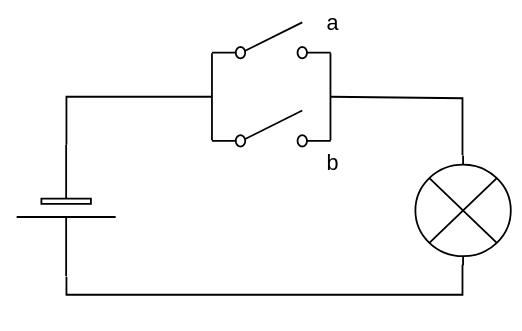
\includegraphics[width=0.8\linewidth]{img/schaltnetz_oder}
		\caption{ODER: $a \vee b$}
		\label{fig:sub1}
	\end{subfigure}%
	\begin{subfigure}{.5\textwidth}
		\centering
		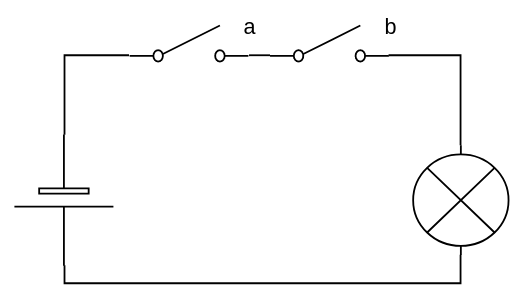
\includegraphics[width=.8\linewidth]{img/schaltnetz_und}
		\caption{UND: $a \wedge b$}
		\label{fig:sub2}
	\end{subfigure}
	\caption{Darstellung zweistelliger Operatoren mit Schaltnetzen}
	\label{fig:test}
\end{figure}

\FloatBarrier
\noindent
\subsubsection{Darstellung mit Wertetabellen}
\begin{table}[h]
	\centering
	\begin{minipage}[b]{0.4\textwidth}
		\centering
		\begin{tabular}{cc|c|c}
			b & a & $a \vee b$ & $a \wedge b$\\ \hline
			0 & 0 & 0 & 0\\
			0 & 1 & 1 & 0\\
			1 & 0 & 1 & 0\\
			1 & 1 & 1 & 1\\
		\end{tabular}
	\end{minipage}
	\begin{minipage}[b]{0.4\textwidth}
		\centering
		\begin{tabular}{c|c}
			$a$ & $\overline{a}$\\ \hline
			0 & 1\\
			1 & 0\\
		\end{tabular}
	\end{minipage}	
	\caption{Wahrheitstabellen für UND/ODER und Negierung}
\end{table}

Ausdrücke der Schaltalgebra (\glqq boolsche Ausdrücke\grqq) bestehen aus:
\begin{itemize}
	\item ein- und zweistelligen Operatoren
	\item Variable (als Platzhalter für einen Wert)
	\item Wert
	\item Klammern
\end{itemize}
\begin{Theorem}{Eingangsbelegung}{}
	Jeder Variable wird ein konkreter Wert zugeordnet
\end{Theorem}
\begin{Theorem}{Ausgangsbelegung}{}
	Der Wert, welcher sich bei einem boolschen Ausdruck bei einer konkreten E-Belegung ergibt, wenn man den boolschen Ausdruck \glqq auswertet\grqq.
\end{Theorem}

Auswertung eines boolschen Ausdrucks: $(a \wedge \neg c) \vee 1 \wedge(b \wedge c) \vee (0 \wedge d)$ (Siehe \reftbl{tab:ausdruck})
\begin{itemize}
	\item Festlegung der E-Belegung
	\item Ersetzen der Variablen durch die entsprechenden Werte
	\item Auswerten \glqq von innen nach außen\grqq
	\subitem Zunächst den Teilausdruck mit der stärksten Bindungskraft, zuletzt der Teilausdruck mit der schwächsten\\ Bindungskraft: am stärksten... $NOT$, Klammer, $AND$, $OR$ ...am schwächsten
	\item bei gleicher Bindungskraft Auswertug von links nach rechts
\end{itemize}

\begin{table}[h!]
\begin{tabularx}{\textwidth}{c|cccc|Y|Y|Y|Y|Y|Y}
	\# & $ d $ & $ c $ & $ b $ & $ a $ & $ \neg c $ & $ a \wedge \neg c $ & $ 1 \wedge (b \wedge c) $ & $ 0 \wedge d $ & $ x \vee y $ & $ f $\\ \hline
	0 & 0 & 0 & 0 & 0 & 1 & 0 & 0 & 0 & 0 & 0\\
	1 & 0 & 0 & 0 & 1 & 1 & 1 & 0 & 0 & 1 & 1\\
	2 & 0 & 0 & 1 & 0 & 1 & 0 & 0 & 0 & 0 & 0\\
	3 & 0 & 0 & 1 & 1 & 1 & 1 & 0 & 0 & 1 & 1\\ \hline
	4 & 0 & 1 & 0 & 0 & 0 & 0 & 0 & 0 & 0 & 0\\
	5 & 0 & 1 & 0 & 1 & 0 & 0 & 0 & 0 & 0 & 0\\
	6 & 0 & 1 & 1 & 0 & 0 & 0 & 1 & 0 & 1 & 1\\
	7 & 0 & 1 & 1 & 1 & 0 & 0 & 1 & 0 & 1 & 1\\ \hline
	8 & 1 & 0 & 0 & 0 & 1 & 0 & 0 & 0 & 0 & 0\\
	9 & 1 & 0 & 0 & 1 & 1 & 1 & 0 & 0 & 1 & 1\\
	10 & 1 & 0 & 1 & 0 & 1 & 0 & 0 & 0 & 0 & 0\\
	11 & 1 & 0 & 1 & 1 & 1 & 1 & 0 & 0 & 1 & 1\\ \hline
	12 & 1 & 1 & 0 & 0 & 0 & 0 & 0 & 0 & 0 & 0\\
	13 & 1 & 1 & 0 & 1 & 0 & 0 & 0 & 0 & 0 & 0\\
	14 & 1 & 1 & 1 & 0 & 0 & 0 & 1 & 0 & 1 & 1\\
	15 & 1 & 1 & 1 & 1 & 0 & 0 & 1 & 0 & 1 & 1\\
\end{tabularx}
\caption{Wahrheitstabelle für $f = (a \wedge \neg c) \vee 1 \wedge (b \wedge c) \vee (0 \wedge d)$}
\label{tab:ausdruck}
\end{table}

\subsubsection{Aus den Huntingtonschen axiomen abgeleitete (beweisbare Gesetze)}
\begin{center}
	\begin{tabular}{ll}
	Assoziativgesetz & $(a \wedge b) \wedge c = a \wedge (b\wedge c)$ \\
	 & $ (a \vee b) \vee c = a \vee (b \vee c) $\\
	Idempotenzgesetz & $ a \wedge a = a $\\
	 & $ a \vee a = a $\\
	Absorptionsgesetz& $ a \wedge (a \vee b) = a $\\
    	& $ a \vee (a \wedge b) = a $\\
    DeMorgan-Gesetz  & $ \overline{(a \wedge b)} = \overline{a} \vee \overline{b} $\\
    				 & $ \overline{(a \vee b)} = \overline{a} \wedge \overline{b} $\\
\end{tabular}
\end{center}
\subsubsection{Beweismethoden}
\begin{itemize}
	\item algebraische Umformungen mit Hilfe der Axiome und bereits bewiesener Gesetze: \\
	$ a \overset{!}{=} a \wedge a $ (Idempotenzgesetz)\\
	$ a \overset{H3}{=} a \wedge 1 \overset{H4}{=} a \wedge ( a \vee \overline{a} ) \overset{H2}{=} (a \wedge a) \vee (a \wedge \overline{a}) \overset{H4}{=} (a \wedge a) \vee 0 \overset{H3}{=} a \wedge a$
	\item Wahrheitstabelle: Terme auf linker und rechter Seite müssen für alle Eingangsbelegugen dieselbe Ausgagsbelegung haben (Tabelle \ref{tab:beweiswhtbl})
	\item spezielle Interpretation von $H4$:\\
	falls $ a \vee \overline{b} = 1 $ und $ a \wedge \overline{b} = 0 $, dann $ a = b $\\
	$ a \vee (b \vee c) \overset{!}{=} (a \vee b) \vee c $ (Assoziativgesetz)
\end{itemize}

\begin{table}[h!]
	\centering
	\begin{tabular}{c|ccc|c|c|c|c}
	\# & c & b & a & $ b \vee c $ & $ a \vee (b \vee c) $ & $ a \vee b $ & $ (a \vee b) \vee c$\\
	0 & 0 & 0 & 0 & 0 & 0 & 0 & 0\\
	1 & 0 & 0 & 1 & 0 & 1 & 1 & 1\\
	2 & 0 & 1 & 0 & 1 & 1 & 1 & 1\\
	3 & 0 & 1 & 1 & 1 & 1 & 1 & 1\\
	4 & 1 & 0 & 0 & 1 & 1 & 0 & 1\\
	5 & 1 & 0 & 1 & 1 & 1 & 1 & 1\\
	6 & 1 & 1 & 0 & 1 & 1 & 1 & 1\\
	7 & 1 & 1 & 1 & 1 & 1 & 1 & 1\\
	 \multicolumn{5}{c}{}& \multicolumn{1}{c}{$\uparrow$}&\multicolumn{1}{c}{}& $\uparrow$\\
	 \multicolumn{5}{c}{}&\multicolumn{3}{c}{gleiche Ausgangsbelegungen}
\end{tabular}
\label{tab:beweiswhtbl}
\caption{Beweis anhand einer Wahrheitstabelle}
\end{table}

$ \overline{a \wedge b} \overset{!}{=} \overline{a} \vee \overline{b}$\\
Beweis: 
\begin{align*}
\overline{\overline{a \vee b}}  \wedge (\overline{a} \vee \overline{b}) \overset{!}{=} 0 \\
\overline{\overline{a \wedge b}} \vee (\overline{a} \vee \overline{b}) \overset{!}{=} 1 \\
\overline{\overline{a \wedge b}} \wedge ( \overline{a} \vee \overline{b}) \overset{\text{dopp. Neg.}}{=} (a \wedge b ) \wedge (\overline{a} \vee \overline{b}) \overset{H2}{=} (a \wedge b) \wedge \overline{a} \vee (a \wedge b) \wedge \overline{b} \\
\overset{H1 \text{ \& AssG.}}{=} b \wedge (a \wedge \overline{a}) \vee a \wedge (b \wedge \overline{b}) \overset{H4}{=} (b \wedge 0) \vee (a \wedge 0) \overset{0-Abs.}{=} 0 \vee 0 \overset{H3 \text{ oder Id.pot.}}{=} 0 \\
\overset{\text{1. Hälfte}}{\blacksquare}
\end{align*}
\begin{align*}
\overline{\overline{a \wedge b}} \vee (\overline{a} \vee \overline{b}) \overset{\text{dopp. Neg.}}{=} (a \wedge b) \vee (\overline{a} \vee \overline{b}) \overset{H2}{=} (a \vee (\overline{a} \vee \overline{b})) \wedge (b \vee (\overline{a} \vee \overline{b})) \\
\overset{H1 \text{ \& AssG.}}{=} ((a\vee \overline{a})\vee \overline{b}) \wedge ((b \vee \overline{b})\vee \overline{a})\\
\overset{H4}{=} (1 \vee \overline{b}) \wedge (1 \vee \overline{a})\\
\overset{\text{1-Absorp.}}{=} 1 \wedge 1 \\
\overset{H3 \text{ oder Id.pot.}}{=} 1\\
\overset{\text{2. Hälfte}}{\blacksquare}
\end{align*}

\noindent
doppelte Negation: $ \overline{\overline{x}} \overset{!}{=} x $\\
Beweis über: $ \overline{\overline{x}} \wedge \overline{x} \overset{!}{=} 0 \text{ und }  \overline{\overline{x}} \vee \overline{x} \overset{!}{=} 1 $\\
\begin{align*}
\begin{array}{cc}
\overline{(\overline{x})} \wedge (\overline{x}) \overset{H4}{=} 0 & \overset{\text{1. Hälfte}}{\blacksquare}\\
\overline{(\overline{x})} \vee (\overline{x}) \overset{H4}{=} 0 & \overset{\text{2. Hälfte}}{\blacksquare}\\
\end{array}
\Bigg\} \blacksquare
\end{align*}
0-Absorption: $ x \wedge 0 \overset{!}{=} 0$\\
Beweis: $ x \wedge 0 \overset{H4}{=} x \wedge (x \wedge \overline{x})  \overset{\text{AssG.}}{=} (x \wedge x) \wedge \overline{x} \overset{\text{Id.pot.}}{=} x \wedge \overline{x} \overset{H4}{=} 0 \blacksquare$\\
\\
1-Absorption: $ x \vee 1 \overset{!}{=} $\\
Beweis: \\
%ToDo
\begin{Theorem}{Boolsche Funktionen}{}
Boolsche Funktionen abhängig von $ n $ Eingangsvariablen: Jeder Eingangsbelegung (der $ n $ Eingangsvariablen) wird genau eine Ausgangsbelegung zugeordnet.
\end{Theorem}

\subsection{Darstellung von Funktionen:}
\begin{enumerate}
	\item algebraischer Funktionsterm
	\item Wahrheitstabelle
\end{enumerate}

\begin{Theorem}{Äquivalenz}{}
	Zwei Funktionen sind äquivalent, wenn sie dieselbe Wahrheitstabelle aufweisen
\end{Theorem}

\begin{Hint}{}{hint}
	Zwei äquivalente Funktionen können durch sehr unterschiedliche Funktionsterme dargestellt werden. (algebraische Umformungen mit Hilfe der Axiome und abgeleiteten Gesetze sind immer möglich)
\end{Hint}
\subsubsection{Funktionen abhängig von Ausgangsvariablen}
\begin{table}[h!]
	\centering
	\begin{tabular}{|r|l|l|}
	\hline
	$ n = 0 $ & $ f_0() = 0 $ & \glqq Nullfunktion\grqq{} \\
					 & $ f_1() = 1 $ & \glqq Einsfunktion\grqq{} \\ \hline
\multicolumn{3}{|l|}{$ \Rightarrow $ (nur) 2 verschiedene Funktionen abhängig von 0 Variablen!}\\ \hline
	$ n = 1 $ & $ f_0(a) = 0 $ & \glqq Nullfunktion\grqq{} \\
					 & $ f_1(a) = \overline{a} $ & \glqq Negation\grqq{} \\
					 & $ f_2(a) = a $ & \glqq Identität\grqq{} \\
					 & $ f_3(a) = 1 $ & \glqq Einsfunktion\grqq{} \\ \hline
 \multicolumn{3}{|l|}{$ \Rightarrow $ genau 4 verschiedene Funktionen abhängig vn 1 Variablen!}\\ \hline
\end{tabular}
\label{tab:funktionenausgang}
\caption{Funktionen abhängig von Ausgangsvariablen ($ n = 0 \ldots 1 $)}
\end{table}
\FloatBarrier

\subsubsection*{Anzahl verschiedener Funktionen?}
Anzahl Zeilen in der Wertetabelle: $ 2^n $\\
Anzahl verschiedener Wertetabellen: $ 2^{2^{n}} \Rightarrow $ Anzahl der Funktionen abhängig von Eingangsvariablen.
\\
\begin{center}
	\begin{minipage}{0.45\textwidth}
	\begin{tabular}{cccl}
		n & $ 2^n $ & $ 2^{2^{n}} $& \\ \cline{1-3}
		0 & 1 & 2 &\\
		1 & 2 & 4 &\\
		2 & 4 & 16&\\
		4 & 16 & 65536&\\
		5 & 32 & $ \approx $ 4 Mrd&\\
		6 & 64 & $ \approx $ 16 Trio & $ \approx $ 1.000.000.000.000.000.000
	\end{tabular}
\end{minipage}
\begin{minipage}{0.2\textwidth}
\fbox{$
	\begin{array}{ccc}
	2^{10} & = & 1024\\
	             & \approx & 1000
	\end{array}
	$}
\end{minipage}
\end{center}

\begin{table}[h]
	\centering
	\begin{tabular}{cc|cccccccccccccccc}
		b & a & $ f_{0} $ & $ f_{1} $ & $ f_{2} $ & $ f_{3} $ & $ f_{4} $ & $ f_{5} $ & $ f_{6} $ & $ f_{7} $ & $ f_{8} $ & $ f_{9} $ & $ f_{10} $ & $ f_{11} $ & $ f_{12} $ & $ f_{13} $ & $ f_{14} $ & $ f_{15} $ \\ \hline
		0 & 0 & 0 & 1 & 0 & 1 & 0 & 1 & 0 & 1 & 0 & 1 & 0 & 1 & 0 & 1 & 0 & 1\\
		0 & 1 & 0 & 0 & 1 & 1 & 0 & 0 & 1 & 1 & 0 & 0 & 1 & 1 & 0 & 0 & 1 & 1\\
		1 & 0 & 0 & 0 & 0 & 0 & 1 & 1 & 1 & 1 & 0 & 0 & 0 & 0 & 1 & 1 & 1 & 1\\
		1 & 1 & 0 & 0 & 0 & 0 & 0 & 0 & 0 & 0 & 1 & 1 & 1 & 1 & 1 & 1 & 1 & 1\\ \hline
		\multicolumn{2}{l|}{$ f(a,b)= $} & 0 & $ \overline{a \vee b} $ & $ \overline{a \Rightarrow b} $ & $ \overline{b} $ & $ \overline{b \Rightarrow a} $ & $ \overline{a} $ & $\overline{a \Leftrightarrow b}$ & $ \overline{a \wedge b} $ & $ a \wedge b $ & $ a \Leftrightarrow b $ & $ a $ & $ b \Rightarrow b $ & $ b $ & $ a \Rightarrow b $ & $ a \vee b $ & $ 1 $\\
		& & \rotatebox{270}{Nullfunktion} & \rotatebox{270}{NOR}&\rotatebox{270}{Inhibition}&\rotatebox{270}{Negation von $ b $}&\rotatebox{270}{Inhibition}&\rotatebox{270}{Negation von $ a $}&\rotatebox{270}{XOR/Antivalenz}&\rotatebox{270}{NAND}&\rotatebox{270}{UND/AND}&\rotatebox{270}{Äquivalenz}&\rotatebox{270}{Identität von $ a $}&\rotatebox{270}{Implikation; aus $ b  $ folgt $ a $}&\rotatebox{270}{Identität von $ b $}&\rotatebox{270}{Implikation: aus $ a $ folgt $ b $}&\rotatebox{270}{ODER/OR}&\rotatebox{270}{Einsfunktion}\\
	\end{tabular}
\label{tab:bolscheoperationen}
\caption{Wahrheitstabelle boolscher Operationen}
\end{table}

\noindent
\textbf{Implikation:} $ a \Rightarrow b $ (\glqq aus a folgt b\grqq)\\
Aussage a: \glqq An der DHBW KA gibt es einen Corona-Fall.\grqq\\
Aussabe b: \glqq An der DHBW KA finden keine Präsenzvorlesungen statt.\grqq\\

\begin{center}
	\begin{tabular}{ccc|c}
	\# & b & a & $ a \Rightarrow b $ \\ \hline
     0 & 0 & 0 & 1\\
     1 & 0 & 1 & 0\\
     2 & 1 & 0 & 1\\
     3 & 1 & 1 & 1\\
\end{tabular}
\end{center}

\begin{Theorem}{Vollständige Operatorensysteme}{}
	Ein vollständiges Operatorensystem (der Boolschen Algebra/Schaltalgebra) ist eine Menge von Operatoren, mit denen jede (Boolsche) Funktion (der Schaltalgebra) dargestellt werden kann.
\end{Theorem}

\begin{table}[h!]
	\centering
	\begin{tabular}{rp{10cm}}
	Satz: & $ \{\wedge, \vee, \neg\} $ ist ein vollständiges Operatorensystem.\\
	Bew.:& Definition der Boolschen/Schaltalgebra.\\ \hline
	Satz: & $ \{\wedge, \neg\} $ ist ein volständiges Operatorensystem.\\
	Bew.:& $ a \vee b \overset{\text{dopp.Neg.}}{=} \overline{\overline{a\vee b}} \overset{\text{De Morgan}}{=} \overline{\overline{a} \wedge \overline{b}}\; \blacksquare$\\ \hline
	Satz: & $ \{\vee, \neg\} $ ist ein vollständiges Operatorensystem.\\
	Bew.:& $ a \wedge b \overset{\text{dopp.Neg.}}{=} \overline{\overline{a \wedge b}} \overset{\text{De Morgan}}{=} \overline{\overline{a} \vee \overline{b}}\; \blacksquare $\\ \hline
	Satz: & $ \overline{\wedge} $ (\glqq NAND\grqq) ist ein vollständiges Operatorensystem.\\
	Bew.: & anhand des vollständigen Operatorensystems $ \{\vee, \neg\}\ldots $
	\newline $ \neg a = \overline{a} \overset{Id.pot.}{=} \overline{(a \wedge a)} \;\overset{\text{1. Hälfte}}{\blacksquare}$
	\newline $ a \vee b \overset{\text{dopp.Neg.}}{=} \overline{\overline{a \vee b}} \overset{\text{De Morgan}}{=} \overline{\overline{a} \wedge \overline{b}} = \overline{\overline{a \wedge a} \wedge \overline{b \wedge b}} \;\overset{\text{2. Hälfte}}{\blacksquare}$\\ \hline
	Satz: & $ \{\overline{\vee}\} $ (\glqq NOR\grqq) ist ein vollständiges Operatorensystem.\\
	Bew.: &anhand des vollständigen Operatorensystems $ \{\vee, \neg\}\ldots $
	\newline $ \neg a = \overline{a} \overset{Id.pot.}{=} \overline{(a \vee a)} \;\overset{\text{1. Hälfte}}{\blacksquare}$
	\newline $ a \wedge b \overset{\text{dopp.Neg.}}{=} \overline{\overline{a \wedge b}} \overset{\text{De Morgan}}{=} \overline{\overline{a} \vee \overline{b}} = \overline{\overline{a \vee a} \vee \overline{b \vee b}} \;\overset{\text{2. Hälfte}}{\blacksquare}$\\ %ToDo
\end{tabular}
\caption{Sätze/Beweise über vollständige Operatorensysteme}
\end{table}

Bsp: Speicherbausteine in \glqq NAND\grqq-Technologie.\\

\begin{Hint}{}{}
	Funktionen können eindeutig durch die Wahrheitstabelle dargestellt werden. Die Darstellung als Funktionsterm ist dagegen nicht eindeutig.\\
	$\Rightarrow$ für jede Funktion gibt es unendlich viele äquivalente Terme!\\
\end{Hint}

\subsubsection*{Wir suchen einen standardisierten Funktionsterm!}
Ausgangspunkt: Wertetabelle\\

\begin{table}[h]
	\centering
	\begin{tabular}{c|ccc|c|cl}
	\# & c & b & a & $ f(a,b,c) $ & Minterm & \\ \hline 
	0 & 0 & 0 & 0 & 1 & $ \overline{c} \overline{b} \overline{a} = (\overline{c} \wedge \overline{b}) \wedge \overline{a}$\tikzmark{minterma} &\multirow{2}{*}{\tikzmark{mintermab}} \\
	1 & 0 & 0 & 1 & 1 & $ \overline{c}\overline{b}a $ \tikzmark{mintermb}\\
	2 & 0 & 1 & 0 & 0 & &\tikzmark{mintermbc}\\
	3 & 0 & 1 & 1 & 1 & $ \overline{c}ba $ \tikzmark{mintermc}&\\
	4 & 1 & 0 & 0 & 0 & &\\
	5 & 1 & 0 & 1 & 0 & & \tikzmark{mintermcd}\\
	6 & 1 & 1 & 0 & 0 & &\\
	7 & 1 & 1 & 1 & 1 & $ cba $ \tikzmark{mintermd}
\end{tabular}
\begin{tikzpicture}[remember picture,overlay]
\draw[-](pic cs:minterma) to (pic cs:mintermab)
node[right] {$ \overline{c}\overline{b} $}; 
\draw[-](pic cs:mintermb) to (pic cs:mintermab); 
\draw[-](pic cs:mintermb) to (pic cs:mintermbc)
node[right] {$ \overline{c}a $}; 
\draw[-](pic cs:mintermc) to (pic cs:mintermbc); 
\draw[-](pic cs:mintermc) to (pic cs:mintermcd)
node[right] {$ ba $}; 
\draw[-](pic cs:mintermd) to (pic cs:mintermcd); 
\end{tikzpicture}
\end{table}

\begin{table}[h!]
	\centering
	\begin{tabular}{lr}
		$ f(a,b,c) = \overline{c}\overline{b}\overline{a} \vee \overline{c}\overline{b}a\vee\overline{c}ba\vee cba  $ & \ac*{DNF}\\
		$ g(a,b,c) = (a\wedge b) \vee (\overline{b} \wedge  \overline{c}) $ & \ac*{DMF}\\
	\end{tabular}
$$ 
\overline{c} \overline{b} \overline{a} \vee \vee \overline{c} \overline{b} a \overset{H2}{=} (\overline{c}\overline{b})\wedge (\overline{a} \ vee  a) \overset{H4}{=} \overline{c} \overline{b} \wedge 1 \overset{H3}{=} \overline{c} \overline{b} 
$$
\end{table}

\begin{itemize}
	\item Ein Literal ist eine Variable in negierter oder nicht-negierter Form
	\item Ein Implikant ist eine Konjunktion von Literalen, für den gilt $ i \implies f $
	\item Ein Minterm ist ein Implikant, bei dem es für jede E-Variable ein Literal gibt. (Auch Vollkonjunktion genannt)
\end{itemize}

\begin{table}[h!]
	\centering
	\begin{tabular}{rp{15cm}}
	Satz: & Ein Minterm hat nur bei einer einzigen E-Belegung \glqq 1\grqq{} als A-Belegung, in allen anderen Fällen der E-Belegung ergibt sich \glqq 0\grqq{} als A-Belegung.\\
	Bew.:& geschenkt (Verständnis)\\ \hline
	Satz: & Die \ac{DNF} der Funktion $ f $ ist ein äquivalent zur Funktion $ f $.\\
	Bew.:& Verständnis/Bildungsregel\\ \hline
	Satz: & Die\ac{DNF} ist (ausgenommen die Reihenfolge der Minterme, sowie die Reihenfolge der Literale in den Mintermen) für eine gegebene Funktion eindeutig.\\
	Bew.:& Bildungsregel \& Wertetabelle ist eindeutig.\\ \hline
	Satz: & Zwei Implikanten einer Funktion lassen sich zu einem Implikanten zusammenfassen, falls:
	\begin{itemize}[itemsep=0mm]
		\item sie ausgenommen ein Literal identisch sind
		\item das sich unterscheidende Literal dieselbe Variable einmal in negierter und einmal in nicht-negierter Form sein muss
	\end{itemize}
	Der Zusammengefasste Implikant ist dann der, welcher durch weglassen des unterschiedlichen Literals entsteht. \\
	Bew.:&$ x \wedge a \vee x \wedge a \overset{H2}{=} x(a \vee \overline{a}) \overset{H4}{=} x1 \overset{H3}{=} x \blacksquare$\\ \hline
	Satz: & Eine \ac{DMF} enthält ausschließlich \ac{PI}.\\
	Bew.:&  Siehe Definition \ref{thm:prim_kernprimimplikant} \\ \hline
	Satz: & Eine \ac{DMF} enthält mindestens alle Kernprimzahlen
\end{tabular}
\end{table}

\begin{Theorem}{\acl*{DNF}}{}
	Die Disjunktion aller Minterme der Funktion $ f $ heißt \ac{DNF}.
\end{Theorem}
\begin{Theorem}{\acl*{PI}}{}
Ein \ac{PI} ist ein Implikant, der mit keinem anderen Implikanten zusammengefasst werden kann
\end{Theorem}
\begin{Theorem}{\acl*{KPI}}{prim_kernprimimplikant}
	Ein \ac{KPI} ist ein \ac{PI}, welcher mindestens eine der Ausgangsbelegung exklusiv abdeckt (bzw. bei dem mindestens ein Minterm beim Zusammenfassen ausschließlich für diesen \ac{PI} verwendet wurde.)
\end{Theorem}

\subsubsection{Schaltnetze}
Siehe Abschnitt \ref{subsec:schaltnetze}.

\subsubsection{KV-Diagramm}
Graphische Darstellung der Ausgangsbelegung
\begin{table}[h!]
\centering
	\begin{tabular}{ccc}
		\# & $ a $ & $ f(a) $\\
		\hline
		0 & 0 & $ f(0) $\\
		1 & 1 & $ f(1) $\\
	\end{tabular}
\quad
	\begin{tabular}{|wc{1cm}|wc{1cm}|}
		$ \overline{a} $ & a \\ \hline
		$ f(0)_{0} $ & $ f(1)_1 $ \\ \hline
	\end{tabular}
\caption{KV-Diagramm mit 1 Variable}
\end{table}
\begin{table}[h!]
	\centering
	\begin{tabular}{c|cc|c}
		\# & b & a & $ f(a,b) $\\ \hline
		0 & 0 & 0 & $ f(0,0) $\\
		1 & 0 & 1 & $ f(0,1) $\\
		2 & 1 & 0 & $ f(1,0) $\\
		3 & 1 & 1 & $ f(1,1) $\\
	\end{tabular}
\quad
	\begin{tabular}{c|c|c|}
		 & $ \overline{a} $  &  $ a $\\ \hline
		 $ \overline{b} $  &  $ f(0,0)_{0} $  &  $ f(1,0)_{1} $ \\ \hline
		 $ b $ & $ f(0,1)_2 $  &  $ f(1,1) _3$ \\ \hline
	\end{tabular}	
\caption{KV-Diagramm mit 2 Variablen}
\end{table}

\begin{table}[h!]
	\centering
	\begin{tabular}{c|c|c|c|c|}
		& $ \overline{a} $ & $ a $ & $ a $ & $ \overline{a} $ \\ \hline
	$ \overline{b} $ & \tikzmark{kv30}{$ 1_0 $} & \tikzmark{kv31}{$ 1_1 $} & $ 0_5 $ & $ 0_4 $\\ \hline
	$ b $ & $ 0_2 $ & \tikzmark{kv33}{$ 1_3 $} & \tikzmark{kv37}{$ 1_7 $} & $ 0_6 $\\ \hline
	\multicolumn{1}{c}{}& \multicolumn{2}{c}{$ \underbrace{\hspace*{\dimexpr2\tabcolsep+1\arrayrulewidth}\hphantom{012}}_{\overline{c}} $}& \multicolumn{2}{c}{$ \underbrace{\hspace*{\dimexpr2\tabcolsep+1\arrayrulewidth}\hphantom{012}}_{c} $}
\end{tabular}
\quad 
$ f(a,b,c) $
\begin{tabular}{cc}
	\textcolor{blue}{$ \blacksquare $} & $ \overline{c}\overline(b) (0+1) $\\
	\textcolor{red}{$ \blacksquare $} & $ \overline{c}a (1+3) $\\
	\textcolor{green}{$ \blacksquare $} & $ ba (3+7) $\\
\end{tabular}
\begin{tikzpicture}[overlay,remember picture]
\draw[blue,rounded corners=5pt] ([xshift=-4pt,yshift=.8em]pic cs:kv30) rectangle ([yshift=-.3em,xshift=14pt]pic cs:kv31);
\draw[red,rounded corners=5pt] ([xshift=-4pt,yshift=.8em]pic cs:kv31) rectangle ([yshift=-.3em,xshift=14pt]pic cs:kv33);
\draw[green,rounded corners=5pt] ([xshift=-4pt,yshift=.8em]pic cs:kv33) rectangle ([yshift=-.3em,xshift=14pt]pic cs:kv37);
\end{tikzpicture}
\caption{KV-Diagramm mit 3 Variablen}
\end{table}
\begin{table}[h!]
	\centering
	\begin{tabular}{c|c|c|c|c|l}
		& $ \overline{a} $ & $ a $ & $ a $ & $ \overline{a} $ &\\ \cline{1-5}
		$ \overline{b} $ & $ \phantom{a}_0 $ & $ \phantom{a}_1 $ & $ \phantom{a}_5 $ & $ \phantom{a}_4 $& \multirow{2}{*}{$\begin{rcases*} \\ \\ \end{rcases*} \overline{d}$}\\ \cline{1-5}
		$ b $ & $ \phantom{a}_2 $ & $ \phantom{a}_3 $ & $ \phantom{a}_7 $ & $ \phantom{a}_6 $ \\ \cline{1-5}
		$ b $ & $ \phantom{a}_{10} $ & $ \phantom{a}_{11} $ & $ \phantom{a}_{15} $ & $ \phantom{a}_{14} $ & \multirow{2}{*}{$ \begin{rcases*} \\ \\ \end{rcases*} d $}\\ \cline{1-5}
		$ \overline{b} $ & $ \phantom{a}_{8} $ & $ \phantom{a}_{9} $ & $ \phantom{a}_{13} $ & $ \phantom{a}_{12} $ \\ \cline{1-5}
		\multicolumn{1}{c}{}& \multicolumn{2}{c}{$ \underbrace{\hspace*{\dimexpr2\tabcolsep+1\arrayrulewidth}\hphantom{012}}_{\overline{c}} $}& \multicolumn{2}{c}{$ \underbrace{\hspace*{\dimexpr2\tabcolsep+1\arrayrulewidth}\hphantom{012}}_{c} $}
	\end{tabular}
	\quad
	\begin{tabular}{rl}
		3: & $ ab\overline{c} \overline{d}$\\
		1: & $ a  \overline{b} \overline{c} \overline{d} $\\
		2: & $ \overline{a} b \overline{c} \overline{d} $\\
		7: & $ abc\overline{d} $\\
	 11: & $ ab\overline{c}d $\\
	 3+7 & $ ab\overline{d} $\\
	 11+15 & $ abd $\\
	 3+7+11+15 & $ ab $\\
	\end{tabular}
\caption{KV-Diagramm mit 4 Variablen}
\end{table}

\FloatBarrier
\noindent
\ac{PI} können im KV-Diagramm gefunden werden, indem wir Bereiche von Feldern mit \glqq 1\grqq-Belegung suchen, welche:
\begin{itemize}
	\item maximal groß sind
	\item rechteckige Form haben
	\item eine 2er-Potenz an Feldern umfassen
\end{itemize}
\acfp*{KPI} erkennt man daran, dass mindestens ein Feld von keinen anderen \ac{PI} abgedeckt wird.\\

\begin{Hint}{}{}
	Zwei benachbarte Felder unterscheiden sich immer in der Belegung genau einer Variable. Nachbarfelder von Randfeldern finden sich am gegenüberliegenden Rand.
\end{Hint}

\begin{table}[h!]
	\centering
	\begin{tabular}{c|c|c|c|c|l}
		& $ \overline{a} $ & $ a $ & $ a $ & $ \overline{a} $ &\\ \cline{1-5}
		$ \overline{b} $ & $ \phantom{a}_0 $ & $ \phantom{a}_1 $ & $ \phantom{a}_5 $ & $ \phantom{a}_4 $& \multirow{2}{*}{$\begin{rcases*} \\ \\ \end{rcases*} \overline{d}$}\\ \cline{1-5}
		$ b $ & $ 1_2 $ & $ {\textcolor{green!80!black}{1}}_3 $ & $ {\textcolor{blue}{1}}_7 $ & $ 1_6 $ \\ \cline{1-5}
		$ b $ & $ 1_{10} $ & $ 1_{11} $ & $ \phantom{a}_{15} $ & $ \phantom{a}_{14} $ & \multirow{2}{*}{$ \begin{rcases*} \\ \\ \end{rcases*} d $}\\ \cline{1-5}
		$ \overline{b} $ & $ \phantom{a}_{8} $ & $ \phantom{a}_{9} $ & $ \phantom{a}_{13} $ & $ 1_{12} $ \\ \cline{1-5}
		\multicolumn{1}{c}{}& \multicolumn{2}{c}{$ \underbrace{\hspace*{\dimexpr2\tabcolsep+1\arrayrulewidth}\hphantom{012}}_{\overline{c}} $}& \multicolumn{2}{c}{$ \underbrace{\hspace*{\dimexpr2\tabcolsep+1\arrayrulewidth}\hphantom{012}}_{c} $}
	\end{tabular}
	\quad
	\begin{tabular}{rlr}
		&& \ac{KPI}\\
		\hcancel[green!80!black]{2+6}: & $ \overline{a} b \overline{d} $ & \hcancel 6\\
		\hcancel[green!80!black]{2+10}:&$ \overline{a} b \overline{c} $ & \hcancel{\phantom{a}}\\
		\hcancel[green!80!black]{11+10}: & $ b\overline{c} d $& \hcancel[green!80!black]{11}\\
		12: & $ \overline{a}\overline{b}cd $ & 12\\
		\multicolumn{3}{l}{DMF: $ \overline{a} b \overline{d} \vee b\overline{c}d \vee \overline{a}\overline{b}cd $}\\
		\hcancel[green!80!black]{\textcolor{blue}{6+7}}: & $ bc\overline{d} $ & \hcancel[green!80!black]7
	\end{tabular}
{\color{green!80!black}
	\begin{tabular}{rlr}
	2+3+6+7: & $ b \overline{d} $ & 6+7/\ac{KPI}\\
	2+3+10+11: & $ b \overline{c} $ & 10+11/\ac{KPI}\\
	\multicolumn{3}{l}{DMF: $ b \overline{d} \vee b \overline{c} \vee \overline{a} \overline{b}cd $}
	\end{tabular}
}
\\
\flushleft
\textcolor{blue}{DMF: $ b \overline{c}d \vee \overline{a} \overline{b} cd \vee bc\overline{d} \vee \overline{a} b \overline{d} = b\overline{c} d \vee \overline{a} \overline{b} c d \vee b c \overline{d} \vee \overline{a} b \overline{d}$}\\
\textcolor{blue}{$\Rightarrow$ Es gibt 2 \ac{DMF}s für diese Funktion $\Rightarrow$ \ac{DMF} nicht eindeutig!}
\end{table}

\textbf{Anmerkung:} 
\begin{itemize}
	\item Eine \ac{DMF}, welche nur aus \acp{KPI} besteht, ist immer eindeutig.
	\item Wenn die \ac{KPI} nicht alle \glqq 1\grqq-Felder abdecken, benötigt man auch einfache \ac{PI} für eine \ac{DMF}.
	\item Für jedes nicht von einem \ac{KPI} abgedeckte \glqq 1\grqq-Feld gibt es immer mindestens 2 \ac{PI}, welche dieses Feld abdecken. (Wenn es nur einen \ac{PI} gäbe, wäre dieser \ac{PI} ein \ac{KPI}!)
	\item Falls ein \ac{PI} für die \ac{DMF} gebraucht wird, kann die \ac{DMF} nicht eindeutig sein; sie kann aber auch eindeutig sein, falls z.B. die beiden fas fehlende Feld abdeckender \ac{PI} unterschiedliche Größe haben.
\end{itemize}

\begin{tabular}{c|c|c|c|c|c|c|c|c|l}
	& $ \overline{a} $ & $ a $ & $ a $ & $ \overline{a} $ & $ \overline{a} $ & $ a $ & $ a $ & $ \overline{a} $ & \\ \cline{1-9}
	$ \overline{b} $ & $ \phantom{a}_0 $ & $ \phantom{a}_1 $ & $ \phantom{a}_5 $ & $ \phantom{a}_4 $ & $ \phantom{a}_{20} $ & $ \phantom{a}_{21} $ & $ \phantom{a}_{17} $ & $ \phantom{a}_{16} $ & \multirow{2}{*}{$\begin{rcases*} \\ \\ \end{rcases*} \overline{d}$}\\ \cline{1-9}
	$ b $ & $ \phantom{a}_2 $ & $ \phantom{a}_3 $ & $ \phantom{a}_7 $ & $ \phantom{a}_6 $ & $ \phantom{a}_{22} $ & $ \phantom{a}_{23} $ & $ \phantom{a}_{19} $ & $ \phantom{a}_{18} $ \\ \cline{1-9}
	$ b $ & $ \phantom{a}_{10} $ & $ \phantom{a}_{11} $ & $ \phantom{a}_{15} $ & $ \phantom{a}_{14} $ &  $ \phantom{a}_{30} $ & $ \phantom{a}_{31} $ & $ \phantom{a}_{27} $ & $ \phantom{a}_{26} $ & \multirow{2}{*}{$ \begin{rcases*} \\ \\ \end{rcases*} d $}\\ \cline{1-9}
	$ \overline{b} $ & $ \phantom{a}_{8} $ & $ \phantom{a}_{9} $ & $ \phantom{a}_{13} $ & $ \phantom{a}_{12} $ & $ \phantom{a}_{28} $ & $ \phantom{a}_{29} $ & $ \phantom{a}_{25} $ & $ \phantom{a}_{24} $ & \\ \cline{1-9}
	\multicolumn{1}{c}{}& \multicolumn{2}{c}{$ \underbrace{\hspace*{\dimexpr4\tabcolsep+1\arrayrulewidth}\hphantom{012}}_{\overline{c}} $}& \multicolumn{2}{c}{$ \underbrace{\hspace*{\dimexpr4\tabcolsep+1\arrayrulewidth}\hphantom{012}}_{c} $}& \multicolumn{2}{c}{$ \underbrace{\hspace*{\dimexpr4\tabcolsep+1\arrayrulewidth}\hphantom{012}}_{\overline{c}} $}& \multicolumn{2}{c}{$ \underbrace{\hspace*{\dimexpr4\tabcolsep+1\arrayrulewidth}\hphantom{012}}_{c} $} & \\
	\multicolumn{1}{c}{}& \multicolumn{4}{c}{$ \underbrace{\hspace*{\dimexpr12\tabcolsep+1\arrayrulewidth}\hphantom{012}}_{\overline{e}} $}& \multicolumn{4}{c}{$ \underbrace{\hspace*{\dimexpr12\tabcolsep+1\arrayrulewidth}\hphantom{012}}_{e} $}&
\end{tabular}
\begin{tabular}{rl}
	3: & $ ab\overline{c}\overline{d}\overline{e} $\\
	19: & $ ab\overline{c}\overline{d}e $ (Nachbar von 3?)\\
\end{tabular}
$\Rightarrow$ KV-Diagramm im 2-dimensionalen: bis 4 E-Variablen, im 3-dimensionalen bis 6 E-Variablen,  ...

\subsubsection{KxF}
\begin{itemize}
	\item Statt DxF (\ac{DNF}, \ac{DMF}) als Disjunktion von Konjunktionen von Literalen gibt es auch KxF (\ac{KNF}, \ac{KMF}) als Konjunktion von Disjunktionen von Literalen.
	\item Statt Feldern und Bereichen mit \glqq 1\grqq-Belegung werden Felder und Bereiche mit \glqq0\grqq-Belegung beschrieben. Diese werden durch Implikate (\ac{PI}, \ac{KPI}, Maxterm, Volldisjunktion) statt Implikanten ($\ldots$) beschrieben.
	\item bei einer mehrheitlichen A-Belegung von 1 ist die/eine KxF sinnvoller als eine DxF, um Transistoren (also Hardware-Aufwand) zu sparen.
\end{itemize}

\newpage
\section{Schaltnetze}
\label{subsec:schaltnetze}
Schaltnetze bestehen aus Gattern und Leitungsverbindungen. Sie sind die Darstellung von Funktionen als Graph, genauer als gerichteter Graph (\glqq Reihenfolge\grqq!)\\
\begin{tabular}{ll}
	Gatter: Knoten & $ \hat{=} $ Operatoren\\
	Leitungsverbindungen: Kanten & $ \hat{=} $ Reihenfolge
\end{tabular}
\begin{figure}[h]
	\centering
	\begin{circuitikz} 
		\draw (0,0) node[european and port] (and) {}
		(and.in 1) node[anchor=east] {a}
		(and.in 2) node[anchor=east] {b}
		(and.out) node[anchor=west]{$ a \wedge b $}
		(and.south) node[below]{AND};
		
		\draw (4,0) node[european or port] (or) {}
		(or.in 1) node[anchor=east] {a}
		(or.in 2) node[anchor=east] {b}
		(or.out) node[anchor=west]{$ a \vee  b $}
		(or.south) node[below]{OR};
		
		\draw (0,-2) node[and port] (aand) {}
		(aand.in 1) node[anchor=east] {a}
		(aand.in 2) node[anchor=east] {b}
		(aand.out) node[anchor=west]{$ a \wedge b $}
		(aand.south) node[below]{Amerikanisches AND};
		
		\draw (4,-2) node[or port] (aor) {}
		(aor.in 1) node[anchor=east] {a}
		(aor.in 2) node[anchor=east] {b}
		(aor.out) node[anchor=west]{$ a \vee b $}
		(aor.south) node[below]{Amerikanisches OR};
		
		\draw (0,-4) node[european buffer port] (ident) {}
		(ident.in 1) node[anchor=east] {a}
		(ident.out) node[anchor=west]{a}
		(ident.south) node[below]{Identer/Identität};
		
		\draw (4,-4) node[european buffer port] (invert) {}
		(invert.in 1) node[anchor=east] {a}
		(invert.out) node[anchor=west]{$ \overline{a} $}
		(invert.bout) node[ocirc, right]{}
		(invert.south) node[below]{Inverter/NICHT};
	\end{circuitikz}
	\caption{Symbole für die Operatoren (\glqq Gatter\grqq) nach DIN/IEC}
\end{figure}

\textbf{Konvetionen:}
\begin{itemize}
	\item Jeder Ein- oder Ausgang eines Gatters kann durch einen nicht-ausgefüllten Kreis invertiert werden.
	\item Eingänge bei Gattern werden meist links (oder alternativ oben) und die Ausgänge meist rechts (oder unten) notiert. Nur in Ausnahmefällen sind Eingänge rechts oder unten bzw. Ausgänge links oder oben!
	\item UND- und ODER-Gatter sind auch mit mehr als zwei (mit beliebig vielen) Eingängen möglich (Abb. \ref{abb:und_verschaltung})
	\item \glqq Verzweigen\grqq{} von Leistungen auf mehrere nachfolgende Gattereingänge ist möglich, in dem an der Verzweigungsstelle ein ausgefüllter Kreis gezeichnet wird
	\item Kreuzungen von Leitungen, die nicht miteinander verbunden sind, sind möglich. An der Kreuzungsstelle darf auch kein ausgefüllter Kreis notiert werden
\end{itemize}

\begin{figure}[h]
	\centering
	\begin{circuitikz}
		\draw 
		(0,0) node[european and port] (A){}
		(A.bin 1) node[ocirc, left]{}
		(A.bin 2) node[ocirc, left]{}
		(A.in 1) node[anchor=east]{c}
		(A.in 2) node[anchor=east]{b}
		(2, -2)node[european and port] (B){}
		(B.bin 2) node[ocirc, left]{}
		(B.in 2) node[anchor=east]{a}
		(A.out) -| (B.in 1)
		(B.out) node[anchor=west]{$ \overline{c}\overline{b}\overline{a} $};
	\end{circuitikz}
	\begin{circuitikz}
		\draw 
		(0,-2) node[european and port] (A){}
		(A.bin 1) node[ocirc, left]{}
		(A.bin 2) node[ocirc, left]{}
		(A.in 1) node[anchor=east]{b}
		(A.in 2) node[anchor=east]{a}
		(2, 0)node[european and port] (B){}
		(B.bin 1) node[ocirc, left]{}
		(B.in 1) node[anchor=east]{c}
		(A.out) -| (B.in 2)
		(B.out) node[anchor=west]{$ \overline{c}\overline{b}\overline{a} $};
	\end{circuitikz}
	\begin{circuitikz}
		\draw node[european and port, number inputs=3] (A){}
		(A.in 1) node[anchor=east]{c}
		(A.in 2) node[anchor=east]{b}
		(A.in 3) node[anchor=east]{a}
		(A.out) node[anchor=west]{$ \overline{c}\overline{b}\overline{a} $};
	\end{circuitikz}
	\caption{Unterschiedliche Darstellungen einer UND-Verschaltung}
	\label{abb:und_verschaltung}
\end{figure}

\begin{figure}[h!]
	\centering
	$$
	f(a,b,c) = \overline{c}\overline{b}\overline{a} \vee \overline{c}\overline{b}a \vee \overline{c}ba \vee cba
	$$
	\begin{circuitikz}
		\draw
		(-2,1) node[anchor=east](inA){a}
		(-1,1) node[anchor=east](inB){b}
		(0,1) node[anchor=east](inC){c}
		(2,0) node [european and port, number inputs=3] (A){}
		(A.bin 1) node[ocirc, left]{}
		(A.bin 2) node[ocirc, left]{}
		(A.bin 3) node[ocirc, left]{}
		(2, -2) node [european and port, number inputs=3] (B){}
		(B.bin 1) node[ocirc, left]{}
		(B.bin 2) node[ocirc, left]{}
		(2, -4) node [european and port, number inputs=3] (C){}
		(C.bin 1) node[ocirc, left]{}
		(2, -6) node [european and port, number inputs=3] (D){}
		(6, -2) node [european or port, number inputs=4] (E){}
		(E.out) node[anchor=west] {$f(a,b,c)$}
		(A.out) -| (E.in 1)
		(B.out) |- (E.in 2)
		(C.out) |- (E.in 3)
		(D.out) -| (E.in 4)
		(inA) |- (A.in 1)
		(inA) |- (B.in 1)
		(inA) |- (C.in 1)
		(inA) |- (D.in 1)
		(inB) |- (A.in 2)
		(inB) |- (B.in 2)
		(inB) |- (C.in 2)
		(inB) |- (D.in 2)
		(inC) |- (A.in 3)
		(inC) |- (B.in 3)
		(inC) |- (C.in 3)
		(inC) |- (D.in 3);
	\end{circuitikz}
	\caption{Realisierung der \ac{DNF} als Schaltnetz}
	\label{dnf:schaltnetz}
\end{figure}

Die Realisierung der \ac{DNF} als Schaltnetz (Abb. \ref{dnf:schaltnetz}) ist meist ungünstig, da es meist \glqq günstigere\grqq{} (weniger Hardware-aufwändige) Schaltnetze für dieselbe Funktion gibt.
\newpage

\subsection{Aufwand}
\begin{itemize}
	\item Hardware-Aufwand
	\item Zeitaufwand (nicht näher behandelt)
\end{itemize}
\subsubsection{Hardware-Aufwand}
\begin{figure}[h!]
	\centering
	\begin{circuitikz}
		\ctikzset{european resistors}
		\ctikzset{noarrowmos}
		\draw
		(0,5) node[anchor=east] (vcc) {+5V}
		(0,5) -- (1,5)  node[circ] {}
		(1,5) -- (1,3)
		(3,3)node[nmos, rotate=-90](mosB){}
		(3,5)node[nmos, rotate=-90](mosA){}
		(1,5) |- (mosA.S)
		(1,3) |- (mosB.S)
		(mosA.G) node[anchor=south]{a}
		(mosB.G) node[anchor=south]{b}
		(mosA.D) -| (5,3) node[circ] {}
		(mosB.D) -| (5,3)
		(5,3) -- (6,3) node[anchor=west]{$a\vee b$};
	\end{circuitikz}
	\caption{ODER}
	\label{abb:mos_or}
\end{figure}
\begin{figure}[h!]
	\centering
	\begin{circuitikz}
		\ctikzset{european resistors}
		\ctikzset{noarrowmos}
		\draw
		(0,5) node[anchor=east] (vcc) {+5V}
		(4,5)node[nmos, rotate=-90](mosB){}
		(1,5)node[nmos, rotate=-90](mosA){}
		(0,5) |- (mosA.S)
		(mosA.D) -- (mosB.S)
		(mosA.G) node[anchor=south]{a}
		(mosB.G) node[anchor=south]{b}
		(mosB.D) -- (5,5) node[anchor=west]{$a\vee b$};
	\end{circuitikz}
	\caption{UND}
	\label{abb:mos_and}
\end{figure}

$\Rightarrow$ wir \glqq messen\grqq{} den Hardware-Aufwand in Anzahl Transistoren.\\ 
Bei UND (Abb. \ref{abb:mos_and}) und ODER (Abb. \ref{abb:mos_or}) brauchen wir so viele Transistoren, wie das Gatter Eingänge hat (bei nicht negierten Ein- und Ausgängen).

\begin{figure}[h!]
	\centering
	\begin{minipage}{0.6\textwidth}
		\begin{circuitikz}
			\ctikzset{european resistors}
			\ctikzset{noarrowmos}
			\draw
			(0,0) node[anchor=south] (vcc){+5V}
			(0,0) -- (0,-1)
			(0,-1) to[R, l_=$R_{\text{Pull-Up}}$] (0,-2)
			(0,-2) -- (0,-3)
			(1,-3)node[nmos, rotate=-90](mosA){}
			(3,-3)node[nmos, rotate=-90](mosB){}
			(0,-2) |- (mosA.S)
			(mosA.D) -- (mosB.S)
			(mosA.G) node[anchor=south]{a}
			(mosB.G) node[anchor=south]{b}
			(mosB.D) |- (4,-3)
			(4,-3) -- (4,-4)
			(4,-4) to[R, l^=$R_{\text{Pull-Down}}$] (4,-5)
			(4,-5) -- (4,-6)
			(4,-6) node[ground]{};
			\draw[red]
			(-0.5,0.5) -- (0.5,-2.5)
			(3.5, -3.5) -- (4.5,-6.5)
			(0,-3) -- (0,-4)
			(0,-4) to[R, color=red, l_=$R_{\text{Pull-Down}}$] (0,-5)
			(0,-5) -- (0,-6)
			(0,-6) node[ground]{}
			(4,0) node[anchor=south] (vcc){+5V}
			(4,0) -- (4,-1)
			(4,-1) to[R, color=red, l^=$R_{\text{Pull-Up}}$] (4,-2)
			(4,-2) -- (4,-3)
			; 
		\end{circuitikz}
	\end{minipage}
	\begin{minipage}{0.3\textwidth}
		mit $R_{\text{Pull-Down}} >> R_{\text{Pull-Up}}$\\
		\textcolor{red}{mit $R_{\text{Pull-Up}} >> R_{\text{Pull-Down}}$}
	\end{minipage}
	\caption{UND \textcolor{red}{negierter Ausgang}}
\end{figure}

\begin{figure}[h!]
	\begin{minipage}{0.4\textwidth}
		\centering
		\begin{circuitikz}
			\draw
			(0,0) node[npn] (Q){}
			(Q.B) node[anchor=east]{Basis}
			(Q.C) node[anchor=west]{Kollektor}
			(Q.E) node[anchor=west]{Emitter}
			;
		\end{circuitikz}\\
		npn-Transistor\\
		schaltet bei positiver Basisspannung durch
	\end{minipage}
	\begin{minipage}{0.4\textwidth}
		\centering
		\begin{circuitikz}
			\draw
			(0,0) node[pnp] (Q){}
			(Q.B) node[anchor=east]{Basis}
			(Q.C) node[anchor=west]{Kollektor}
			(Q.E) node[anchor=west]{Emitter}
			;
		\end{circuitikz}\\
		pnp-Transistor\\
		schaltet bei negativer Basisspannung durch
	\end{minipage}
	\caption{NPN und PNP-Transistor}
\end{figure}
\clearpage
\noindent
$\Rightarrow$ negierte Eingänge durch Ersetzen der üblichen npn-Transistoen durch pnp-Transistoren\\
$\Rightarrow$ auch bei negierten Eingängen reicht ein Transistor je Eingang\\
\\
nMOS: Realisierung nur mit npn-Transistoren\\
pMOS: Realisierung nur mit pnp-Transistoren\\
$\Rightarrow$ früher gängige Realisierungstechnologien\\
heute: CMOS: (\textbf{C}omplimentary \textbf{M}etal \textbf{O}xide \textbf{S}miconductor)\\
\hspace*{2em} Realisierung jedes Eingang durch 2 Transistoren (ein npn- und ein pnp-Transistor)\\
\hspace*{2em} jeweils ein Transistor zeiht wechselweise nach oben oder nach unten\\
\\
$\Rightarrow$ der Einfachheit halber trotzdem:\\
\hspace*{2em} bei UND und ODER (\glqq Elementargatter\grqq) entspricht die Anzahl der Eingänge der Anzahl dafür notwendiger Transistoren (nur zu Vergleichszwecken eingesetzt)

\subsubsection{Schaltnetzanalyse}
\begin{figure}[h!]
	\centering
	$$
	g(a,b,c) = (a\wedge b) \vee(\overline{b} \vee \overline{c})
	$$
	\begin{minipage}{0.4\textwidth}
		\begin{circuitikz}
			\draw
			(0,2) node[anchor=east](inA){a}
			(0,1) node[anchor=east](inB){b}
			(0,0) node[anchor=east](inC){c}
			(3,0) node[european and port](a1){}
			(3,2) node[european and port](a2){}
			(a1.bin 1) node[anchor=east,ocirc]{}
			(a1.bin 2) node[anchor=east,ocirc]{}
			(inA) |- (a2.in 1)
			(inB) |- (1,1) node[circ]{}
			(1,1) |- (a2.in 2)
			(1,1) |- (a1.in 1)
			(inC) |- (a1.in 2)
			(5,1) node[european or port](o){}
			(a2.out) |- (o.in 1)
			(a1.out) |- (o.in 2)
			(a2.out) node[anchor=west]{x}
			(a1.out) node[anchor=west]{y}
			(o.out) node[anchor=west]{$ g(a,b,c) $}
			;
		\end{circuitikz}
	\end{minipage}
	\begin{minipage}{0.3\textwidth}
		\begin{tabular}{c|ccc|cc|c}
			\# & c & b & a & x & y & $ x \vee y = g(a, b, c) $\\ \hline
			0 & 0 & 0 & 0 & 0 & 1 & 1\\
			1 & 0 & 0 & 1 & 0 & 1 & 1\\
			2 & 0 & 1 & 0 & 0 & 0 & 0\\
			3 & 0 & 1 & 1 & 1 & 0 & 1\\
			4 & 1 & 0 & 0 & 0 & 0 & 0\\
			5 & 1 & 0 & 1 & 0 & 0 & 0\\
			6 & 1 & 1 & 0 & 0 & 0 & 0\\
			7 & 1 & 1 & 1 & 1 & 0 & 1\\
			
		\end{tabular}
	\end{minipage}
	\label{abb:schaltnetzG}
	\caption{}
\end{figure}

Im Schaltnetz (Abb. \ref{abb:schaltnetzG}) ist $ g $ äquivalent zu $ f $ (Abb. \ref{dnf:schaltnetz})! Für die Realisierung von $ g $ sind aber nur 6 Transistoren nötig, d.h. 10 Transistoren weniger als für $ f $.\\
\\
Wie finden wir eine weniger aufwändige Realisierung als die \ac{DNF}?\\
\begin{Theorem}{\acl*{DMF}}{}
	Eine \ac{DMF} ist eine Disjunktion von Konjunktionen von Literalen, welche die Funktion darstellt und \glqq minimal\grqq{} ist.\\
	Minimal bedeutet, mit am wenigsten Hardware-Aufwand zu realisieren.
\end{Theorem}

\newpage
\section{Schaltwerke}
\begin{tabular}{ll}
	Verhalten: & Können sich etwas merken/\glqq speichern\grqq\\
	Afubau: & Rückkopplungen (von Aus- zu Eingängen) sind erlaubt \\
\end{tabular}

\begin{figure}[h!]
	\centering
	
	\begin{circuitikz}
		\draw
		(0,2) node[anchor=east](inA){a}
		(0,0) node[anchor=east](inB){b}
		(3,0) node[european or port](o1){}
		(3,2) node[european or port](o2){}
		(o1.bout) node[anchor=west,ocirc]{}
		(o2.bout) node[anchor=west,ocirc]{}
		(inA) |- (o2.in 1)
		(inB) |- (o1.in 2)
		
		(o1.out) |- (3,0.75)
		(o2.out) |- (3,1.25)
		(1,0.75) |- (o1.in 1)
		(1,1.25) |- (o2.in 2)
		(1,0.75) -- (3,1.25)
		(1,1.25) -- (3,0.75)
		
		(5,2) node[anchor=west](outx){x $ \; \; x = \overline{a \vee y'} $}
		(5,0) node[anchor=west](outy){y $ \; \; y = \overline{b \vee x'} $}
		
		(o2.in 1) node[anchor=north east]{y'}
		(o1.in 2) node[anchor=south east]{x'}
		(o2.out) |- (outx)
		(o1.out) |- (outy)
		;
	\end{circuitikz}
\caption{Beispielschaltung zur Schaltwerksanalyse}
\label{abb:schaltwerk1}
\end{figure}

\subsection{Schaltwerksanalyse}
\begin{enumerate}
	\itemsep0em
	\item Auftrennen der Rückkopplung und \glqq Neubenennen\grqq{} der bislang rückgekoppelten Eingänge
	\item Aufstellen der Wertetabelle, wobei die vormals rückgekoppelten Eingänge zuerst (ganz links) notiert werden.
	\item Notieren von stabilen und instabilen Zeilen der Wertetabelle, wobei bei den stabilen Zeilen die Belegung der rückgekoppelten Eingänge der Belegung der entsprechenden Ausgänge entspricht.
	\item Bei instabilen Tabellenzeilen wird die Folgezeile notiert, indem die E-Belegung durch die entsprechende A-Belegung ersetzt wird, bis wir entweder eine stabile Zeile erreichen, oder ein Zustand zweimal vorkommt (Kreislauf!)
	\item Benennen der Zustände anhand der Belegung der rückgekoppelten Eingänge
	\item Aufstellen eines Zustandsübergangsdiagramms
	\item Interpretation des Zustandsübergangsdiagramms, um ein \glqq sinnvolles\grqq, \glqq schlüssiges\grqq{} Verhalten festzustellen.
\end{enumerate}

\begin{table}[h!]
	\centering
	$y = \overline{b \vee x'} \;\; x = \overline{a \vee y'}$
	\\[1em]
	\begin{tabular}{c|cc|cc|cc|l}
		\# & y'  & x'  & b & a & y & x & \\ \hline
		0 & 0 & 0 & 0 & 0 & 1 & 1 & \xmark $\rightarrow$ 12 $\rightarrow$ 0 \textcolor{red}{\lightning}\\
		1 & 0 & 0 & 0 & 1 & 1 & 0 & \xmark $\rightarrow$ 9 \cmark \\
		2 & 0 & 0 & 1 & 0 & 0 & 1 & \xmark $\rightarrow$ 6 \cmark\\
		3 & 0 & 0 & 1 & 1 & 0 & 0 & \cmark \\ \cline{2-3}
		4 & 0 & 1 & 0 & 0 & 0 & 1 & \cmark\\
		5 & 0 & 1 & 0 & 1 & 0 & 0 & \xmark $\rightarrow$ 1 $\rightarrow$ 9 \cmark\\
		6 & 0 & 1 & 1 & 0 & 0 & 1 & \cmark\\
		7 & 0 & 1 & 1 & 1 & 0 & 0 & \xmark $\rightarrow$ 3 \cmark\\ \cline{2-3}
		8 & 1 & 0 & 0 & 0 & 1 & 0 & \cmark\\
		9 & 1 & 0 & 0 & 1 & 1 & 0 & \cmark\\
		10 & 1 & 0 & 1 & 0 & 0 & 0 & \xmark $\rightarrow$ 2 $\rightarrow$ 6 \cmark\\
		11 & 1 & 0 & 1 & 1 & 0 & 0 & \xmark $\rightarrow$ 3 \cmark\\ \cline{2-3}
		12 & 1 & 1 & 0 & 0 & 0 & 0 & \xmark $\rightarrow$ 0 $\rightarrow$ 12 \textcolor{red}{\lightning}\\
		13 & 1 & 1 & 0 & 1 & 0 & 0 & \xmark $\rightarrow$ 1 $\rightarrow$ 9 \cmark\\
		14 & 1 & 1 & 1 & 0 & 0 & 0 & \xmark $\rightarrow$ 2 $\rightarrow$ 6 \cmark\\
		15 & 1 & 1 & 1 & 1 & 0 & 0 & \xmark $\rightarrow$ 3 \cmark\\
	\end{tabular}
\caption{Wahrheitstabelle der Schaltwerksanalyse für Abbildung \ref{abb:schaltwerk1}}.
\end{table}
\begin{figure}[h!]
	\centering
	\begin{tikzpicture}[->,>=stealth',shorten >=1pt, line width=2pt, 
node distance=4cm, style ={minimum size=20mm}]
\tikzstyle{every node}=[font=\huge]
\node [circle, draw] (a) {00};
\node [circle, draw] (b) [below left=of a] {01};
\node [circle, draw] (c) [below right=of a] {10};
\node [circle, draw] (d) [below right=of b]{11};
\path  (a) edge [loop above] node [above=-0.7cm]{11} (a);
\path  (b) edge [loop left] node {10+00} (b);
\path  (c) edge [loop right] node {01+00} (c);

 \path (a) edge                    node [below=-0.7cm]{10}     (b)
                edge                    node [below=-0.7cm]{01}    (c)
                edge [bend left]   node [above=-0.7cm]{00}   node [at end] {\textcolor{red}{\lightning}} ++(4,2)
          (b) edge [bend left]    node [above=-0.7cm]{11}    (a)
                edge                     node [near start, above=-1cm]{01}   (c)
          (c) edge [bend right]  node [above=-0.7cm]{11}    (a)
                edge [bend left]    node [near start, below=-0.7cm]{10} (b)
          (d) edge [bend left]     node [below=-0.7cm]{10}    (b)
                edge [bend right]  node [below=-0.7cm]{01}    (c)
                edge                     node [near end, right=-1cm]{11}  (a)
                edge [bend right]  node [below=-0.7cm]{00} node [at end] {\textcolor{red}{\lightning}} ++(4,-2)
           ;
\end{tikzpicture}
\caption{Zustandsübergangsdiagramm (gerichteter Graph)}
\end{figure}
\subsection{FlipFlops}
\subsubsection{RS-FF: Reset-Set-Flip-Flop (Abbildung \ref{abb:schaltwerk1})}
\begin{tabularx}{\textwidth}{llX}
	\multicolumn{3}{l}{\textbf{1-bit-Speicherbaustein}}\\
	\multicolumn{2}{l}{\textbf{2 Arbeitszustände}:} & 10 gesetzt\\
	\multicolumn{2}{l}{}& 01 rückgesetzt\\
	\textbf{Ausgänge}: & Q & Zustand\\
	& Q* & invertierter Zustand\\
	\textbf{Eingänge}: & S & Setzeingang\\
	& R & Rücksetzeingang\\
	\textbf{Verhalten}: &\multicolumn{2}{l}{R = 0 \& S = 0: Arbeitszustand bleibt erhalten}\\
	& \multicolumn{2}{l}{R = 0 \& S = 1: FF wird gesetzt}\\
	& \multicolumn{2}{l}{R = 1 \& S = 0: FF wird rückgesetzt}\\
	& \multicolumn{2}{l}{R = 1 \& S = 1: verbotene Eingangsbelegung, um unerwünschten Zustand 00 nicht zu erreichen}\\
	\multicolumn{3}{l}{\textbf{Weitere Zustände}:}\\
	& 00 & unerwünscht, soll nicht erreicht werden, da bei E-Belegung R=S=0 ein Zustandsflimmern statt Zustand beibehalten eintritt.\\
	& 11 & wird nie stabil, sondern nur beim Zustandsflimmern immer nur kurzzeitig erreicht.
\end{tabularx}
\\[1em]
\textbf{Schaltsymbol}:\\
\begin{center}
	\begin{circuitikz}
		\tikzset{rs-ff/.style={flipflop, flipflop def={t1=R, t3=S, t6={Q*},t4=Q}}}
		\draw
		node[rs-ff]{};
	\end{circuitikz}
\end{center}

\textbf{Anwendung RS-FF}\\
Lichtschalter mit 2 Tastern für An und Aus (Aus $\hat{=}$ Not-Aus)\\

\subsubsection{2. FF-Typ: D-FF (\glqq Data\grqq)}
Nur einen D-Eingang über den das FF sowohl gesetzt als auch rückgesetzt werden kann. (bei D=1: FF wird gesetzt, bei D=0 FF wird rückgesetzt)

\begin{figure}[h!]
	\centering
	\begin{circuitikz}
\tikzset{rs-ff/.style={flipflop, flipflop def={t1=R, t3=S, t6={Q*},t4=Q}}}
\draw
node[european buffer port](not){}
(not.bout) node[anchor=west,ocirc]{}
node[rs-ff,right=1cm of not, anchor=pin 1](RS){}
(RS.pin 3) to[short, -*] ++(-3.5,0) coordinate(punkt)
(punkt) to[short] ++(-1,0) coordinate(n)
(n) node[anchor=east]{D}
(not.in) -| (punkt)
(RS.pin 6) to[short] ++(3,0) coordinate(qs)
(RS.pin 4) to[short] ++(3,0) coordinate(q)
(qs) node[anchor=west]{Q*}
(q) node[anchor=west]{Q}
(RS.pin 1) -- (not.out)
;
\end{circuitikz}
\\ etwas aufwändige Realisierung für eine einfache Leitung: \\
\begin{circuitikz}
	\draw
	(0,0) node[anchor=east](d){D}
	(0,0) to[short] ++(10,0) coordinate(q)
	(q) node[anchor=west]{Q}
	;
\end{circuitikz}
\caption{Ersatzschaltbild D-FlipFlop}
\end{figure}

$\Rightarrow$ Wir brauchen einen Takt!

\begin{Theorem}{Taktsteuerung}{}
	Die Schaltung übernimmt die E-Belegung/ändert die A-Belegung nur bei aktivem Takt. Bei inaktivem Takt hat die E-Belegung keine Auswirkung auf die A-Belegung/die A-Belegung ändert sich nicht.
\end{Theorem}

\begin{Hint}{}{}
	Ein Schaltnetz mit Taktsteuerung wird zum Schaltwerk, da es die A-Belegung und/oder E-Belegung beim letzten aktiven Takt speichern und solange ausgeben muss, bis der Takt inaktiv ist.
\end{Hint}

\subsection{Taktsteuerung}
\subsubsection{\acf{TPS}}
\begin{itemize}
	\vspace*{-0.5em}
	\itemsep 0em
	\item \textbf{positive \ac{TPS}:} Der Takt ist aktiv, solange der Takt den Pegel \glqq 1\grqq{} hat.
	\item\textbf{negative \ac{TPS}:} Der Takt ist aktiv, solange der Takt den Pegel \glqq 0\grqq{} hat.
\end{itemize}

\subsubsection{\acf{TFS}}
\begin{itemize}
	\vspace*{-0.5em}
	\itemsep 0em
	\item \textbf{positive \ac{TFS}:} Der Takt ist aktiv, wenn der Takt von Pegel \glqq 0\grqq{} auf \glqq 1\grqq{} wechselt.
	\item \textbf{negative \ac{TFS}:} Der Takt ist aktiv, wenn der Takt von Pegel \glqq 1\grqq{} auf \glqq 0\grqq{} wechselt.
\end{itemize}

\begin{figure}[h!]
	\centering
	
	\begin{circuitikz}
		\tikzset{rs-ff/.style={flipflop, flipflop def={t1=R, t3=S, t6={Q*},t4=Q}}}
		\draw
		node[european and port](a1){}
		node[rs-ff,right=1cm of a1, anchor=pin 1](RS){}
		node[european and port,below=0.75cm of a1](a2){}
		(a1.in 1) to[short] ++(-3,0) coordinate(er)
		(a2.in 2) to[short] ++(-3,0) coordinate(es)
		(a1.in 2) to[short,] ++(-0.5,0) coordinate(p1)
		(p1) to[short, -*] ++(0,-0.5) coordinate(p2)
		(a2.in 1) -| (p2)
		(p2) to[short] ++(-2.5,0) coordinate(et)

		(er) node[anchor=east]{R}
		(et) node[anchor=east]{T}
		(es) node[anchor=east]{S}
		
		(RS.pin 6) to[short] ++(3,0) coordinate(qs)
		(RS.pin 4) to[short] ++(3,0) coordinate(q)
		(qs) node[anchor=west]{Q*}
		(q) node[anchor=west]{Q}
		(RS.pin 1) |- (a1.out)
		(RS.pin 3) |- (a2.out)
		
		(a1.bin 2) node[color=red,anchor=east,ocirc]{}
		(a2.bin 1) node[color=red,anchor=east,ocirc]{}
		;
	\end{circuitikz}
\caption{Realisierung des RS-FlipFlop mit positiver \ac{TPS} \textcolor{red}{negativer \ac{TPS} (invertierter Takt)}}
\end{figure}
\begin{figure}[h!]
	\centering
	\begin{circuitikz}
		\tikzset{flipflop AB/.style={flipflop,
				 flipflop def={t1=R, t3=S, t4=Q, t6={Q*},
				 c2=1,  t2={\texttt{C}}},
				 }}
			 \draw
			 node[flipflop AB]{};
	\end{circuitikz}
\begin{circuitikz}
\tikzset{flipflop AB/.style={flipflop,
		flipflop def={t1=R, t3=S, t4=Q, t6={Q*},
			c2=1,  t2={\texttt{C}}},
}}
\draw[color=red]
node[flipflop AB](a){}
(a.bpin 2) node[anchor=east,ocirc]{}
;
\end{circuitikz}
\caption{Schaltsymbol RS-FlipFlop mit positiver \ac{TPS} \textcolor{red}{negativer \ac{TPS}}}
\end{figure}

\subsubsection{Schaltnetzanalyse}
\begin{minipage}{0.45\textwidth}
	\centering
	\begin{circuitikz}
\draw
node[european buffer port](N){}
node[european and port, right=1cm of N, anchor=in 1](A){}
(N.bout) node[ocirc, anchor=west] {}
(N.in) to[short, -*] ++(0, -1) coordinate(punkt)
(punkt) -| (A.in 2)
(punkt) to[short] ++(-2,0) coordinate(punkt2)
(punkt2) node[anchor=east] {a (T)}
(N.out) -- (A.in 1)
;
\end{circuitikz}
\end{minipage}
\begin{minipage}{0.45\textwidth}
	\centering
	\begin{tabular}{c|c|c|c}
		\# & a & x & $ a \wedge x $\\
		0 & 0 & 1 & 0\\
		1 & 1 & 0 & 0\\
	\end{tabular}
\end{minipage}
\\ \\
\textbf{Zeitverhalten:}\\
\begin{tikztimingtable}[timing/slope=0, scale=4]
	a     	& LLLLHHHHHHLLLLLL\\
	x 	     & HHHHHLLLLLLHHHHH\\
	f(a)   	& LLLLLLHLLLLLLLLL \\
	\extracode
	\makeatletter
	\tikzset{
		timing/z/.style={color=red},
		timing/l/.style={color=red},
		timing/h/.style={color=red}
	}
\end{tikztimingtable}

\subsubsection{Realisierung RS-FF mit positiver \ac{TFS} (\glqq TFS für Arme\grqq)}

\begin{minipage}{0.6\textwidth}
		\begin{circuitikz}
			\tikzset{flipflop AB/.style={flipflop,
					flipflop def={t1=R, t3=S, t4=Q, t6={Q*},
						c2=1,  t2={\texttt{T}}},
			}}
		\draw
		node[european buffer port](N){}
		node[european and port, right=0.5cm of N, anchor=in 1](A){}
		node[flipflop AB, right=0.5cm of A, anchor=pin 2](FF){}
		(A.out) -| (FF.pin 2)
		(N.bout) node[ocirc, anchor=west] {}
		(N.in) to[short, -*] ++(0, -0.75) coordinate(punkt)
		(punkt) -| (A.in 2)
		(punkt) to[short] ++(-2,0) coordinate(punkt2)
		(punkt2) node[anchor=east] {T}
		(N.out) -- (A.in 1)
		(FF.pin 1) to[short] ++(-7,0)
		(FF.pin 3) to[short] ++(-7,0)
		;
	\end{circuitikz}
\end{minipage}
\begin{minipage}{0.35\textwidth}
	\begin{itemize}
		\item[$\bigoplus$]  sehr geringer HW-Aufwand
		\item[$\bigominus$] Problem ist das Zeitverhalten: Reicht die positive TP von T mod aus, um das nachfolgende FF zum Schalten zu bringen? 
	\end{itemize}
\end{minipage}
\\
\glqq bessere\grqq/\glqq sicherere\grqq, aber auch \glqq teurere\grqq Variante einer \ac{TFS}:\\
\begin{itemize}
	\vspace*{-0.5em}
	\itemsep 0em
	\item doppelte Anzahl an \glqq internen\grqq Zuständen
	\subitem Für jeden TP jeweils ein Zustand
	\item nur beim Wechsel von \glqq 0\grqq- auf \glqq 1\grqq-Zustand darf sich die A-Belegung ändern.
\end{itemize}

\begin{figure}[h!]
	\centering
	\begin{circuitikz}
		\tikzset{flipflop AB/.style={flipflop,
				flipflop def={t1=R, t3=S, t4=Q, t6={Q*},
					c2=1,  t2={\texttt{T}}},
		}}
	   \draw node[flipflop AB](A){};
	   \draw[color=red] node[flipflop AB,right=1cm of A]{};
	\end{circuitikz}
\caption{Schaltsymbol RS-FF mit pos. TFS / \textcolor{red}{neg. TFS}}
\end{figure}

Damit: D-FF mit pos. TPS: (neg. TPS sowie pos. \& neg. TFS entsprechend)

\begin{figure}[h!]
\centering
	\begin{circuitikz}
	\tikzset{flipflop AB/.style={flipflop,
			flipflop def={t1=R, t3=S, t4=Q, t6={Q*},
				c2=1,  t2={\texttt{T}}},
	}}
	\draw
	node[european buffer port](N){}
	node[flipflop AB, right=0.5cm of N, anchor=pin 2](FF){}
	(N.out) |- (FF.pin 1)
	(N.bout) node[ocirc, anchor=west] {}
	(N.in) to[short, -*] ++(0, -0.75) coordinate(punkt)
	(punkt) -| (FF.pin 3)
	(punkt) to[short] ++(-2,0) coordinate(punkt2)
	(punkt2) node[anchor=east] {D}
	;
	\end{circuitikz}
\caption{Ersatzschaltbild für ein D-FlipFlop mit Taktflankensteuerung}
\end{figure}

\FloatBarrier
\noindent
Schaltsymbol:\\
\begin{figure}[h!]
	\centering
	\begin{circuitikz}
			\tikzset{flipflop D/.style={flipflop,
				flipflop def={t3=D, t4=Q, t6={Q*},
					c2=1,  t2={\texttt{T}}},
		}}
		\draw node[flipflop D]{};
	\end{circuitikz}
\caption{Schaltsymbol D-FlipFlop}
\end{figure}

\FloatBarrier
\noindent
\textbf{Anwendung:} manche 1bit-Speicherzellen im Computer z.B. CPU-Register, Teil des \glqq CPU-Cache\grqq{} (insbesondere L1-Cache) -- nicht dagegen im Hauptspeicher

\subsection{Erneut FlipFlops}
\subsubsection{JK-FlipFlop (Jack Kilby,  Jump and Kill)}

Verhalten wie RS-FlipFlop, aber keine verbotene Eingangsbelegung, d.h. J=K=1 ist explizit erlaubt!

\begin{figure}[h!]
	\centering
	
	\begin{circuitikz}
		\tikzset{rs-ff/.style={flipflop, flipflop def={t1=R, t3=S, t6={Q},t4={Q*}}}}
		\draw
		node[european and port](a1){}
		node[rs-ff,right=1cm of a1, anchor=pin 1](RS){}
		node[european and port,below=0.75cm of a1](a2){}
		(a1.in 2) to[short] ++(-3,0) coordinate(er)
		(a2.in 1) to[short] ++(-3,0) coordinate(es)
		
		(a1.in 1) to[short,] ++(0,0.5) coordinate(p1)
		(a2.in 2) to[short] ++(0,-0.5) coordinate(p2)
		
		(er) node[anchor=east]{K}
		(es) node[anchor=east]{J}
		
		(RS.pin 6) to[short, -*] ++(1,0) coordinate(qs)
		(RS.pin 4) to[short, -*] ++(1,0) coordinate(q)
		(qs) to[short] ++(1,0)
		(q) to[short] ++(1,0)
		(p1) -| (qs)
		(p2) -| (q)
		
		(RS.pin 1) |- (a1.out)
		(RS.pin 3) |- (a2.out)
		
		;
	\end{circuitikz}
	\caption{JK-FlipFlop Ersatzschaltbild mit RS-FlipFlop}
\end{figure}

\FloatBarrier
\noindent
Was passiert bei $ J=K=1 $? Das JK-FF wechselt seinen Zustand (es \glqq toggelt\grqq), solange $ J=K=1 $ (also mehrfach).\\

\textbf{Unterschied zu RS-FF:}\\
\begin{itemize}
	\itemsep 0em
	\vspace*{-0.5em}
	\item[] Zustandswechsel tritt bei $ J=K=1 $ auf (und nicht bei $ R=S=0 $),
	\subitem also dann, wenn ich das FF gleichzeitig setzen und rücksetzen will (was unmöglich ist), wohingegen das RS-FF dann \glqq flimmert\grqq, wenn es seinen Zustand (bei $ R=S=0 $) nicht ändern sollte!
	\item[] JK-FF mit \ac{TPS}: FF toggelt, solange $ J=K=T=1 $!
	\item[] JK-FF mit \ac{TFS}: FF toggelt, wenn $ J=K=1 $ und akt. TF! und außerdem genau 1x! (\textbf{Achtung:} bei \glqq TFS für Arme\grqq{} kann das nicht sichergestellt werden!)
\end{itemize}

\subsubsection{T-FlipFlop (Toggle)}
$\Rightarrow$ Besitzt nur einen Takteingang\\
$\Rightarrow$ Nur mit \ac{TFS}, da es bei aktiver TF genau 1x toggelt.\\
\\
\textbf{Realisierung:}\\
\begin{minipage}{0.4\textwidth}
	\centering
	\begin{circuitikz}
	\tikzset{flipflop JK/.style={flipflop,
		flipflop def={t1=K,t3=J,t4=Q,c2=1, t2={\texttt{T}}},
	}}
	\draw node[flipflop JK](JK){}
	(JK.pin 1) to[short] ++(-0.5,0) coordinate (e1)
	(JK.pin 3) to[short] ++(-0.5,0) coordinate (e2)
	(JK.pin 2) to[short] ++(-2,0) coordinate (et)
	(e1) node[anchor=east]{\glqq 1\grqq}
		(e2) node[anchor=east]{\glqq 1\grqq}
	(et) node[anchor=east]{T}
	;
\end{circuitikz}
\end{minipage}
oder
\begin{minipage}{0.4\textwidth}
	\centering
\begin{circuitikz}
	\tikzset{flipflop JK/.style={flipflop,
			flipflop def={t3=D,t6=Q,t4={Q*},c2=1,t2={\texttt{T}}},
	}}
	\draw node[flipflop JK](JK){}
	(JK.pin 2) to[short] ++(-2,0) coordinate (et)
	(JK.pin 3) to[short] ++(0,-0.75) coordinate(p)
	(JK.pin 4) to[short] ++(2,0) coordinate (p1)
	(p) -| (JK.pin 4)
	(et) node[anchor=east]{T}
	(p1) node[anchor=west]{Q}
	;
\end{circuitikz}
\end{minipage}
\\
\vspace*{2em}

\begin{figure}[h!]
	\centering
	\begin{circuitikz}
	\tikzset{flipflop T/.style={flipflop,
			flipflop def={t4=Q,c2=1,t2={\texttt{T}}},
	}}
	\draw node[flipflop T](T){}
	(T.pin 2) to[short] ++(-2,0) coordinate (et)
	(T.pin 4) to[short] ++(2,0) coordinate (p1)
	(et) node[anchor=east]{T}
	(p1) node[anchor=west]{Q}
	;
\end{circuitikz}
\begin{tikztimingtable}[timing/slope=0, scale=5]
	T     	& LHLHLHL\\
	Q 	   & LHHLLHH\\
\end{tikztimingtable}
\caption{Verhalten eines T-FlipFlops}
\end{figure}

\noindent
$\Rightarrow$Frequenzalbierer\\
$\Rightarrow$(Licht-)Schalter, welcher bei jeder Betätigung umgeschaltet wird.

\begin{center}
	\begin{circuitikz}
	\tikzset{flipflop T/.style={flipflop,
			flipflop def={t4=Q,c2=1,t2={\texttt{T}}},
	}}
	\draw
	node[flipflop T](T1){}
	node[flipflop T, right=1cm of T1](T2){}
	node[flipflop T, right=1cm of T2](T3){}
	(T1.pin 4) |- (T2.pin 2)
	(T2.pin 4) |- (T3.pin 2)
	(T1.pin 2) node[anchor=east] {$ T $}
	(T1.pin 4) node[anchor=north] {$ Q_0 $}
	(T2.pin 4) node[anchor=north] {$ Q_1 $}
	(T3.pin 4) node[anchor=north] {$ Q_2 $}
	;
\end{circuitikz}
\end{center}
\begin{center}
	\begin{tabular}{ccccccccr}
		T & $ Q_0 $ & $ Q_1 $ & $ Q_2 $ &  & $ Q_2 $ & $ Q_1 $ & $ Q_0 $ & \\
		0 & 0 & 0 & 0 &  & 0 & 0 & 0 & \\
		1 & 1 & 1 & 1 &  & 1 & 1 & 1 & 7\\
		0 & 1 &  & 1 &  &  &  &  & \\
		1 & 0 & 1 & 1 &  & 1 & 1 & 0 & 6\\
		0 & 0 & 1 & 1 &  &  &  &  & \\
		1 & 1 & 0 & 1 &  & 1 & 0 & 1 & 5\\
		0 & 1 & 0 & 1 &  &  &  &  & \\
		1 & 0 & 0 & 1 &  & 1 & 0 & 0 & 4\\
		0 & 0 & 0 & 1 &  &  &  &  & \\
		1 & 1 & 1 & 0 &  & 0 & 1 & 1 & 3\\
		0 & 1 & 1 & 0 &  &  &  &  & \\
	\end{tabular}
\\
$\Rightarrow$ Rückwärtszähler\\
$\Rightarrow$ Vorwärtszähler bei Invertierung zwischen Q und T
\end{center}

\vspace*{2em}
\begin{center}
	\begin{circuitikz}
		\tikzset{flipflop T/.style={flipflop,
				flipflop def={t4=Q,c2=1,t2={\texttt{T}}},
		}}
		\draw
		node[flipflop T](T1){}
		node[european xor port, right=1cm of T1](T2){}
		node[flipflop T, right=1cm of T2](T3){}
		(T1.pin 4) |- (T2.in 2)
		(T2.out) |- (T3.pin 2)
		(T2.in 1) |- ++(0,1) coordinate(p1)
		(T1.pin 2) node[anchor=east] {$ T $}
		(p1) node[anchor=south] {direction}
		;
	\end{circuitikz}
\end{center}

\begin{tabular}{rl}
	XOR: & bei \textit{direction=1} wird das andere E-Signal invertiert\\
	          & bei \textit{direction=0} nicht invertiert\\
	$\Rightarrow$ & Zähler, der in beide Richtungen (vor- und rückwärts) zählen kann\\
	\multicolumn{2}{l}{Noch zu verbessern:}\\
	& Auch bei Änderung von \textit{direction} wird \glqq gezählt\grqq\\
	& Setz- bzw. Rücksetzmöglichkeit\\
\end{tabular}
\\
Der Hardware-Aufwand für ein D-FF als 1bit-Speicher ist (zu) groß!

\begin{center}
	\begin{circuitikz}
		\draw
		(0,1) node[anchor=east](inT){T}
		(3,0) node[european and port](a1){}
		(3,2) node[european and port](a2){}

		(inT) |- (1,1) node[circ]{}
		(1,1) |- (a2.in 2)
		(1,1) |- (a1.in 1)

		
		(5,0) node[european or port](o1){}
		(5,2) node[european or port](o2){}
		(o1.bout) node[anchor=west,ocirc]{}
		(o2.bout) node[anchor=west,ocirc]{}
		(a2.out) |- (o2.in 1)
		(a1.out) |- (o1.in 2)
		(o1.out) |- (5,0.75)
		(o2.out) |- (5,1.25)
		(3,0.75) |- (o1.in 1)
		(3,1.25) |- (o2.in 2)
		(3,0.75) -- (5,1.25)
		(3,1.25) -- (5,0.75)
		(6,2) node[anchor=west](outx){}
		(6,0) node[anchor=west](outy){}
		(o2.out) |- (outx)
		(o1.out) |- (outy)
		;
				
		\draw
		node[european buffer port, left=1cm of a2](not){}
		(not.bout) node[anchor=west,ocirc]{}
		(a1.in 2) to[short, -*] ++(-3.5,0) coordinate(punkt)
		(punkt) to[short] ++(-1,0) coordinate(n)
		(n) node[anchor=east]{D}
		(not.in) -| (punkt)
		(a2.in 1) -| (not.out)
		;
	\end{circuitikz}
\\
$\Rightarrow$ 8Tr.\\
\end{center}


\begin{center}
	\begin{circuitikz}
		\draw
		
		
		(5,0) node[european and port, number inputs=3](o1){}
		(5,2) node[european and port, number inputs=3](o2){}
		(o1.bout) node[anchor=west,ocirc]{}
		(o2.bout) node[anchor=west,ocirc]{}
		(o2.bin 1) node[ocirc]{}
		(o1.out) |- (5,0.75)
		(o2.out) |- (5,1.25)
		(3,0.75) |- (o1.in 1)
		(3,1.25) |- (o2.in 3)
		(3,0.75) -- (5,1.25)
		(3,1.25) -- (5,0.75)
		(6,2) node[anchor=west](outx){}
		(6,0) node[anchor=west](outy){}
		(o2.out) |- (outx)
		(o1.out) |- (outy)
		(1,1) node[anchor=east](inT){T}
		
		(inT) |- (2,1) node[circ]{}
		(2,1) |- (o2.in 2)
		(2,1) |- (o1.in 2)
		;
		
		\draw
		(o1.in 3) to[short, -*] ++(-3.5,0) coordinate(punkt)
		(punkt) to[short] ++(-1,0) coordinate(n)
		(n) node[anchor=east]{D}
		(o2.in 1) -| (punkt)
		;
	\end{circuitikz}
\\
$\Rightarrow$ 6Tr.\\
\end{center}

\subsubsection{Anderes Speicherprinzip: Kondensator Speicherladung}
\begin{tabular}{ll}
	Kondensator \glqq aufgeladen\grqq: & \glqq 1\grqq\\
	Kondensator entladen: &  \glqq 0\grqq\\
\end{tabular}
\\ \vspace*{2em}
\FloatBarrier
\begin{minipage}{0.45\textwidth}
	\centering
	\begin{circuitikz}[scale=6]
		\draw (0,0) to[C] ++(0,-0.5) coordinate(g)
		(g) node[tlground]{}
		(0,0) -- (0.5,0);
		\draw[color=blue]
		[<->] (0.5,0) -- (0.5,-0.5) node[midway, right] {U}
		;
	\end{circuitikz}
\end{minipage}
\begin{minipage}{0.45\textwidth}
	\textbf{Einspeichern/schreiben:}\\
	Anlegen der Betriebsspannung für \glqq 1\grqq \\
	Anlegen von $ 0V $ für \glqq 0\grqq\\
\textbf{	Lesen:}\\
	Betriebsspannung $\Rightarrow$ \glqq 1\grqq\\
	\glqq$ 0V $\grqq{} $\Rightarrow$ \glqq 0\grqq
\end{minipage}

\textbf{Realisierung:} Zwei kurze Stücke \glqq Leiterbahnen\grqq{} parallel geführt.\\
$\Rightarrow$ Prinzip \glqq Plattenkondensator\grqq\\
$\Rightarrow$ Aufwand im IC entspricht etwa einem Transistor.

\begin{center}
	\begin{circuitikz}[scale=3]
		\draw
		node[nmos, rotate=-90](mosA){}
		(mosA.D) node[anchor=west]{data}
		(mosA.G) node[anchor=south]{select}
		(mosA.S) to[C] ++(0,-0.5) coordinate(g)
		(g) node[tlground]{}
		;
	\end{circuitikz}
\end{center}

Nur bei \textit{select = 1} wird der Kondensatorspeicher angesprochen, und zwar lesen oder schreiben wir ihn abhängig davon, ob wir die Spannung messen, oder eine Spannung anlegen!\\
$\Rightarrow$ HW-Aufwand: 2 Transistor-Äquivalente, also $ \dfrac{1}{3} $ des HW-Aufwands für ein D-FF!\\
\\
\textbf{Nachteile:}\\
\begin{enumerate}
	\item Ladung geht beim Lesen verloren\\
	$\Rightarrow$ Wieder einschreiben nach jedem Lesen nötig. \glqq Refresh-Logik\grqq{} notwendig, d.h. für jedes gleichzeitig gelesene Bit benötigen wir zusätzlich ein D-FF.\\
	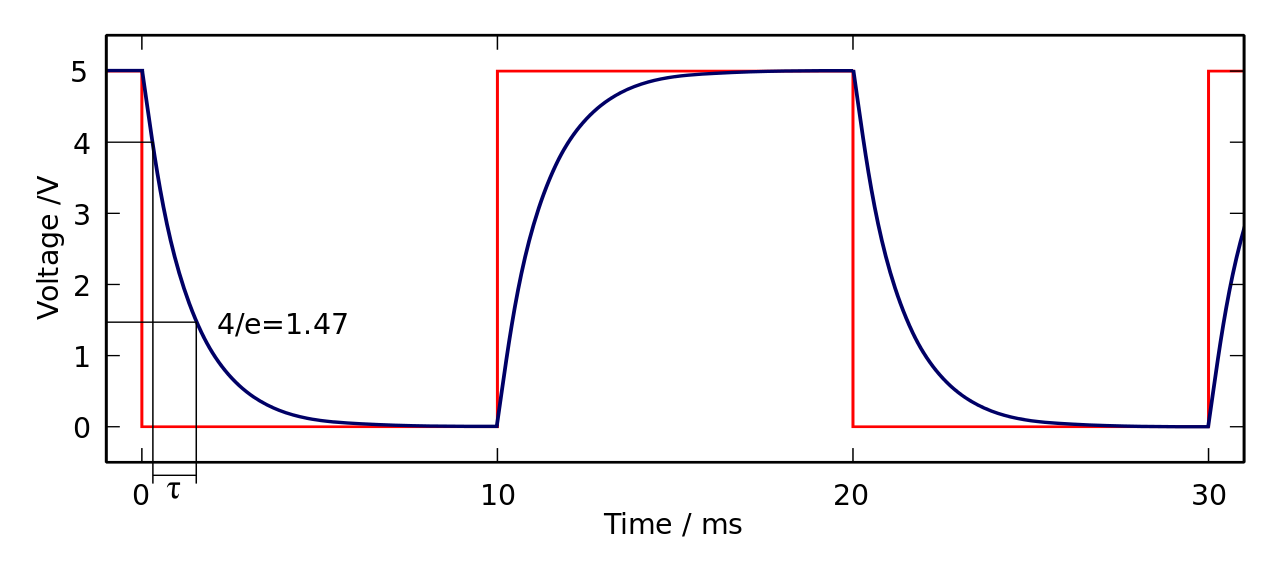
\includegraphics[width=0.7\textwidth]{img/cap}\footnote{\href{https://commons.wikimedia.org/wiki/File:Capacitor_Square_wave_charge-discharge.svg}{Wikipedia}}
	\item langsame Zugriffsgeschwindigkeit beim Schreiben aufgrund Lade-/Entlade-Kurve des Kondensators
	\item Lesen geht eigentlich schnell, aber ab dem zweiten Lesen muss auf das Wiedereinschreiben nach dem ersten Lesen gewartet werden \textcolor{red}{$\Rightarrow$ Zugriffsgeschwindigkeit ist auch ab dem zweiten Lesen recht langsam!}
	\item Aufgrund von Leckströmen verliert der Kondensator ständig (langsam/ein wenig) Ladung\\
	$\Rightarrow$ auch ohne explizites Lesen muss der Kondensatorspeicher nach einiger Zeit wiederaufgefrischt werden.\\
	$\Rightarrow$ zyklisches komplettes Durchlesen des gesamten Speichers führt zu einem Refresh jeder Speicherzelle\\
	$\Rightarrow$ während eines laufenden Refreshzyklus dauert der Zugriff unverhältnismäßig länger als \glqq normal\grqq
\end{enumerate}

Einsatz: \glqq DRAM\grqq{} $\hat{=}$ Dynamic RAM $\hat{=}$ Kondensatorspeicher\\
$\Rightarrow$ Hauptspeicher, L3-Cache, heutige Grafikkartenspeicher (meist)\\
\\
dem gegenüber \glqq SRAM\grqq{} $\hat{=}$ Static RAM $\hat{=}$ D-FF-Speicher\\
$\Rightarrow$ CPU-Register, L1-Cache, früherer teurer Grafikkartenspeicher

\newpage
\pagenumbering{roman}
\tcblistof{def}{Definitionsverzeichnis}
\newpage
\section{Abkürzungsverzeichnis}
\begin{acronym}[Bash]
	\acro{SWS}{Stellenwertsysteme}
	\acroplural{SWS}[SWS]{Stellenwertsysteme}
	\acro{FKZ}{Festkommazahl}
	\acroplural{FKZ}[FKZ]{Festkommazahlen}
	\acro{GKZ}{Gleitkommazahl}
	\acroplural{GKZ}[GKZ]{Gleitkommazahlen}
	\acro{BCD}{Binary Coded Decimal}
	\acro{BBB}{Bandbreitenbedarf}
	\acro{NRZ}{Non-Return-to-zero}
	\acro{RZ}{Return-to-Zero}
	\acro{AMI}{Alternate Mark Inversion}
	\acro{TRG}{Taktrückgewinnung}
	\acro{GSF}{Gleichspannungs-/stromfreiheit}
	\acro{SSH}{Störsicherheit}
	\acro{DNF}{Disjunktive Normalform}
	\acro{DMF}{Disjunktivie Minimalform}
	\acro{KNF}{Konjunktive Normalform}
	\acro{KMF}{Konjunktive Minimalform}
	\acro{KPI}{Kernprimimplikant}
	\acroplural{KPI}[KPI]{Kernprimipimplikanten}
	\acro{PI}{Primimplikant}
	\acro{TFS}{Taktflankensteuerung}
	\acro{TPS}{Taktpegelsteuerung}
\end{acronym}
\end{document}